\pagebreak
\chapter{MP-PIC: Multiphase Particle-in-Cell Method}
\label{ch:MPPIC}
In this chapter, we discuss the theoretical background of the \MP (Multi‑Phase Particle‑In‑Cell) method. We look at the governing equations and how they are solved and at the modeling approaches, especially at the methods used for the particles.
Subsequently, the first numerical implementation of the \MP method is discussed, following the formulation originally presented by O'Rourke and Snider in \cite{MPPICFirst}.
 
% an overview of approaches used for modeling gas-solid multiphase flows. Then we will look at one in detail, the \MP method, the governing equation and how they are solved numerically. 
% This chapter is mainly based on the paper which first presented the \MP method \cite{MPPICFirst}.

%TODO: von wo aus anfangen? Euler/Euler bzw. Euler/Lagrange Modelle erklären?

\section{Governing equations}
In the \MP method, the fluid phase is described using an Eulerian, therefore continuous framework, whereas the particle phase is represented using a Lagrangian, therefor discrete, approach. 
For the fluid phase mass and momentum equations are solved. 
For a reactive solver we would need to also solve species and energy equations.
The particle phase is governed by the Liouville equation for the distribution function of particle positions, velocities and sizes.
For the particle behavior we look at the first and second moment of the Liouville equation.
Obtained particle properties are projected on to an Eulerian grid, where they are used to compute the solid stress tensor.
The stress tensor models particle-particle interactions and in addition to further Eulerian properties we use them to advance the particle positions.
In this section we will look at the governing equation for both phases as well as the interpolation operators that couple them and the numerical solution.
\subsection{Fluid Phase}
The fluid phase, in our case gas, is modeled through an Eulerian approach for incompressible flows.
The gas phase is governed by the conservation equations for mass
\begin{equation}
    \dfrac{\partial (\fvf \rf)}{\partial \tvar} + \nabla \cdot (\fvf \rf \uf) = 0,
\end{equation}
and momentum
\begin{equation}
    \label{eq:momEul}
    \dfrac{\partial (\fvf \rf \uf)}{\partial \tvar} + \nabla \cdot (\fvf \rf \uf \uf) = - \nabla \p -\nabla \cdot (\fvf \fst)  - \boldsymbol{F} + \fvf \rf \g.
\end{equation}
%\todo[color = kit-blue!60, inline]{der viscous stress $\nabla \cdot (\fvf \fst)$ ist in anderen Papern \cite{mathMPPIC} nur $\nabla \cdot \fst$. Scheint ein häufigeres Problem zu sein \cite{differentTau}.}
Here $\uf$ is the fluid velocity and $\fvf$ the fluid volume fraction.
If not labeled otherwise, the gradient refers to the spatial component.
In the momentum term
%\Todo{Stimmen die Vorzeichen?}
%\Todo{Wie viel soll hier zu Herleitung EL?}
%To achieve multiphase coupling, we will later insert a source term. \Todo{Probably}. 
we have $t$ as time, $\p$ as fluid pressure and $\fst$ as the fluid stress tensor. $\F$ is the interphase momentum transfer, which will be discussed in the following subsection. 
For both equations we assume that we have no interphase mass transfer.
The fluid stress tensor was omitted from the equations in the original series of papers that presented the method \cite{MPPICFirst}, \cite{MP2d},\cite{MPInterpolation}, therefore setting it to zero
\begin{equation}
\label{eq:FlStTeZero}
    \fst = 0,
\end{equation}
which is also assumed in this chapter. %The term is again discussed in the \OF implementation as this term only matches the implementation if the condition above \eqref{eq:FlStTeZero} is fulfilled.
In later papers \cite{chimera},the fluid stress tensor is defined by the Newtonian viscosity law
\begin{equation}
    \label{eq:fst}
    \fst = - \fv \left( \nabla \uf + ( \nabla \uf)^T \right) + \dfrac{2}{3} \fv ( \nabla \cdot \uf),
\end{equation}
see \cite{mathMPPIC}.
We also assume that we have an ideal gas, which we will use later in the implicit approximations. Therefore the pressure can be related to the fluid density by
\begin{equation}
\label{eq:gasDensReal}
    \dfrac{\p}{\rf^\gamma} = constant.
\end{equation}

\subsection{Solid Phase}
The solid phase is treated as both a continuous phase as well as a discrete phase in the \MP method.
The behavior of the particles is governed by the Liouville equation for the particle probability distribution function.
We look at the distribution of the velocities among a sufficient number of particles in a domain $\Omega \subset \R^3$, with velocity points in the velocity space $\Pi \subset \R^3$. 
The number density of particles in a volume $\x \in \Omega$, with a velocity $\u \in \Pi$, mass $\m$ at time $\tvar$ is given by the particle probability distribution function
\begin{equation}
    \pd : \Omega \times \Pi \times I \times \R \to \R^+, \qquad (\x, \u, \tvar, \m) \mapsto \pd (\x , \u , \tvar, \m).  
\end{equation}
% with $\xp$ the particle position, $\up$ the particle velocity, $\Op$ the particle volume, $\m$ the particle mass and $\rp$ the particle mass density.

% Consider the domain $\Omega \subset\R^3$, %partial volume $\Omega_p \subset \R^3$ 
% velocity space $\Pi \subset \R^3$ and time interval $I = [0,\T], \ \T \in \R$. For the solid phase we define a particle distribution function %$\pd: \Omega \times \Pi \times \Op \times I \times \R \times \R \to \R^+, \ \pd(\xp, \up, \Op, t, \rp, \m) $


%Assuming that the particle Volume and particle density are constant, the particle distribution function quantifies the average number of particles having velocity $\up$ at $\xp$ with particle mass $\m$ at time $\tvar$.
The particle density function gives the probable average number of particles per unit volume $\Np$ with a velocity in the interval $(\Vp, \Vp + \Delta \Vp)$ and mass in the interval $(\M, \M + \Delta \M)$ when integrating over the velocity and mass
%\Todo{Ahhhh why is it called distribution and not density}
\begin{equation}
    \Np = \int_{\M}^{\M+\Delta \M} \int_{\Vp}^{\Vp + \Delta \Vp} \pd d \up d \m. 
\end{equation} 
For a small volume this can be approximated by
\begin{equation}
    \Np \approx \pd (\xp , \Vp , \tvar, \M) \cdot \Delta \Vp \cdot \Delta M.
\end{equation}
The definition of the probability particle density function is of a probabilistic nature.
The probable number of particles in the given volume the number of particles with a velocity in and a mass of $\m$ at time $\tvar$ is not necessarily contained since fluctuations can occur but is the average number of particles when the time $dt$ is smoothed out.
In the following we will assume that $\pd$ is not negative, finite, continuous and goes to zero as the velocity becomes infinite.

The solids volume fraction is then given by taking particles of all mass and velocities
\begin{equation}
    \label{eq:svf}
    \pvf = \MultiIntegral{2} \pd \dfrac{\m}{\rp} d \m d \up.
\end{equation}
% The particle size is given by
% \begin{equation}
%     N(\boldsymbol{x}_p, \boldsymbol{v}_p, \Omega_p, t, \rho_p, m_p) = \int f(\boldsymbol{x}_p, \boldsymbol{v}_p, \Omega_p, t, \rho_p, m_p) dv_p.
% \end{equation}
With the sum of the fluid volume fraction and the particle volume fraction being equal to one.

We assume that the total number of particles near $\xp$ with velocity $\up$ in any volume is conserved. Therefor we have
\begin{equation}
\label{eq:partConservation}
    \dfrac{d}{dt} \MultiIntegral{2} \pd d \up d \xp = 0.
\end{equation}
%By applying the Leipniz integral rule and, using that the volume over which we integrate is arbitrary, we transform the equation above into the Liouville equation.
Using that the this hold for all volumes we can transform the equation above into what the authors refer to as a Liouville equation
%\todo[inline,color=kit-blue!60]{Die Liouville Gleichung ist eigentlich für die Hamiltonische Mechanik definiert und müsste Divergenz frei und Konservativ sein. Ist sie halt hier nicht..., aber who cares?}
\begin{align}
    \dfrac{\partial \pd}{\partial \tvar} + \dfrac{\partial}{\partial \xp} \left( \pd \dfrac{d \xp}{d \tvar} \right)+ \dfrac{\partial}{\partial \up} \left( \pd \dfrac{d \up}{d \tvar} \right) = 0 \\
    \label{eq:Liouville}
    \Leftrightarrow \dfrac{\partial \pd}{\partial \tvar} + \dfrac{\partial (\pd \up)}{\partial \xp} + \dfrac{\partial (\pd \Ap)}{\partial \up} = 0. % \left( \dfrac{\partial f}{\partial t} \right)_{coll}.
\end{align}
%The Liouville equation was originally derived for Hamiltonian mechanics which would require it to be conservative ($\nabla_\u \cdot \Ap)$ and divergence free $\nabla \cdot \up = 0$, which is not fulfilled in our case.
%The term has used 
%To avoid confusion, we will keep referring to the equation as the Liouville equation. \Todo{Quelle einfügen}
Here $\Ap$ is the particle acceleration. The term is defined by Newton's equations of motion. The forces acting on the particle are aerodynamic drag, pressure gradient, interparticle stress and gravity.
The equations are given by
\begin{align}
    \dfrac{d \xp}{d \tvar} &= \up, \\
    \label{eq:accel}
    \Ap = \dfrac{d \up}{d \tvar} &=\d(\uf - \up) - \dfrac{1}{\rp} \nabla \p - \dfrac{1}{\pvf \rp} \nabla \scs + \g.
\end{align}
%Op particle volume
Here $\uf$ is the flow fluid velocity, $\d(d_p,\up, \xp,\tvar)$ is the drag function, discussed in Sec. \ref{sec:MPDrag}, $\scs(\xp, \tvar)$ is the solids contact stress, discussed in Eq. \ref{eq:solidStress} and $\p$ is the mean flow fluid thermodynamic pressure and $d_p$ is the particle diameter.
We account for the effects of collisions by the spatial gradient of the solid stress. 
Adding collision terms on the right hand side of the Liouville Eq. \eqref{eq:Liouville} we can model the behavior of particles after a collision more locally
\begin{equation}
    \label{eq:LiouCollide}
    \dfrac{\partial \pd}{\partial \tvar} + \dfrac{\partial (\pd \up)}{\partial \xp} + \dfrac{\partial (\pd \Ap)}{\partial \up} = \left( \dfrac{\partial \pd}{\partial 
    \tvar} \right)_{coll},
\end{equation}
see \cite{damp}, \cite{isotropy}.
We will cover these damping terms later in this chapter, see Sec. \ref{sec:damping}.

To derive the interphase momentum transfer function we take the moments from the Liouville equation \eqref{eq:Liouville}.
We multiply the equation by $\m$ and integrate over the mass and velocity. This yields a connection between the field properties and the interaction between the two phases called the particle conservation equation
\begin{equation}
\begin{aligned}
    \MultiIntegral{2} \m \left( \dfrac{\partial \pd}{\partial \tvar} + \nabla \cdot (\pd \up) + \nabla_{\up} \cdot (\pd \Ap)\right) d \up d \m = 0 \\
    \Leftrightarrow
    \dfrac{\partial }{\partial \tvar} \MultiIntegral{2} \pd \m d \m d \up + \nabla \cdot \left( \MultiIntegral{2} m \pd \up d\up d \m \right) = 0\\
    \stackrel{\eqref{eq:svf}}{\Leftrightarrow} \dfrac{\partial (\pvf \rp )}{\partial t} + \nabla \cdot (\pvf \rp \overline{\up}) = 0    
\end{aligned}    
\end{equation}
with the third term, the acceleration term, being zero by using integration by parts and $\pd \to 0$ for $\lvert \up \rvert \to \infty$.
The term for the mean particle velocity is given by
\begin{equation}
    \overline{\up} = \dfrac{1}{\rp \pvf}\MultiIntegral{2} \pd \m \up d\m d \up.
\end{equation}

%In this case our particle distribution function depends only on particle position, velocity, mass and time. 
%For a particle distribution function that instead of the mass would depend on the density and volume we would need to integrate over these factors.
We obtain the second momentum term by multiplying the Liouville Eq. \eqref{eq:Liouville} by $\m \cdot \up$ and again integrating over $\m$ and \up
\begin{equation}
\label{eq:mom2Begin}
    \MultiIntegral{2} \m \up \left( \dfrac{\partial \pd}{\partial \tvar} + \nabla_{\xp} \cdot (\pd \up) + \nabla_{\up} \cdot \left(\pd
    \left(\d(\uf - \up) - \dfrac{1}{\rp} \dfrac{\partial \p}{\partial \xp} - \dfrac{1}{\pvf \rp} \dfrac{\partial \scs}{\partial \xp} + \g \right)
    \right)\right) d \up d \m = 0
\end{equation}
% \begin{equation}
% \label{eq:mom2Begin}
%     \MultiIntegral{2} \m \up \left( \dfrac{\partial \pd}{\partial \tvar} + \nabla \cdot (\pd \up) + \nabla_{\up} \cdot \Ap \right) d \up d \m = 0
% \end{equation}
With partial integration and using again that $\pd \to 0$ for $\lvert \up \rvert \to \infty$ we have
\begin{equation}
    \MultiIntegral{2} \m \up \nabla_{\up} \cdot (\pd \Ap ) d \up d \m = - \MultiIntegral{2} \m \Ap \pd d \up d \m.
\end{equation}
Using the mean particle velocity to reformulate
\begin{equation}
    \MultiIntegral{2} \m \up \dfrac{\partial \pd}{\partial \tvar} d \up d \m = \dfrac{\partial}{\partial \tvar} (\rp \pvf \overline{\up} )
\end{equation}
and
\begin{equation}
    \MultiIntegral{2} \m \up \up \pd d \up d \m = \rp \overline{\up} \overline{\up} + \MultiIntegral{2} \m (\up - \overline{\up}) ( \up - \overline{\up}) \pd d \up d \m.
\end{equation}
By replacing the corresponding terms in equation \eqref{eq:mom2Begin} and multiplying by $\pvf \rp$ we then have the particle momentum equation
\begin{equation}
    \begin{aligned}
\label{eq:secondMomentum}
    %\MultiIntegral{2} \m \up \left( \dfrac{\partial \pd}{\partial \tvar} \right. & \left.+ \nabla_{\xp} \cdot (\pd \up) + \nabla_{\up} \cdot \left(\pd
    %\left(\d(\uf - \up) - \dfrac{1}{\rp} \dfrac{\partial \p}{\partial \xp} - \dfrac{1}{\pvf \rp} \dfrac{\partial \scs}{\partial \xp} + \g \right)
    %\right)\right) d \up d \m = 0 \\
    %\Leftrightarrow 
    \dfrac{\partial ( \pvf \rp \overline{\up})}{\partial t} &+ \nabla_{\xp} \cdot (\pvf \rp \overline{\up} \overline{\up} ) + \nabla \scs + \pvf \nabla \p \\ &= \pvf \rp \g + \MultiIntegral{2} \pd \m \d (\uf - \up) d \m d\up - \nabla \cdot \left[ \MultiIntegral{2} \pd \m (\up - \overline{\up}) (\up - \overline{\up}) d \m d \up \right].
    \end{aligned}
\end{equation}
The last term on the right hand side in the equation mimics the kinematic stress from the particle velocity fluctuations, similar to Reynold stress. The last terms on both the left and right hand side of the equation depend on both phases and therefor contribute to the interphase momentum transfer function, which models the particle force per unit volume on the fluid phase
%\Todo{Second momentum term}
\begin{equation}
    \label{eq:InterMomTrans}
    \F = \MultiIntegral{2} \pd \m [\d (\uf - \up) - \dfrac{1}{\rp} \nabla \p] d\m d\up.
\end{equation}
We can split the integral up into two terms. The first represents the momentum exchange due to aerodynamic drag.
%For more detailed models we can use particle density and volume instead of mass.
In the gas momentum equation \eqref{eq:momEul} the pressure gradient is multiplied by the gas volume fraction. This term arises from the second term in \eqref{eq:InterMomTrans}, as shown by the following calculation.
We know that for the volume fraction
\begin{equation}
    \fvf + \pvf = 1 \qquad \nabla p - \fvf \nabla p = \pvf \nabla p
\end{equation}
holds.
From equation \eqref{eq:svf} we have
\begin{equation}
    \fvf \nabla p =  \int \int \pd \m \dfrac{1}{\rp} \nabla \p d\m d\up
\end{equation}
which is included in equation \eqref{eq:InterMomTrans} in the interface momentum transfer function. 
By setting both terms against one another only $\pvf \nabla p$ remains in the equation \eqref{eq:InterMomTrans}.

% In later versions, the \MP method was extended to two-dimensional problems and a scheme for three-dimensional models was introduced. 
% On top of that a collision term was added on the right hand side of the Liouville equation. 
% The collision operator in general reads


\subsection{Interphase Drag Model}
\label{sec:MPDrag}
%\Todo{Something with Gidaspow}
Investigation of flow through fixed beds has led to several empirical models to predict the pressure drop, which correlates to the drag force. 


Several different models have been suggested for the \MP method. 
In the paper that first presented the method \cite{MPPICFirst} the interphase drag model was used 
\begin{align*}
    D_p = C_D\dfrac{3}{8} \dfrac{\rf}{\rp} \dfrac{\lvert \uf - \up \rvert}{r_p}
\end{align*}
with the Drag constant
\begin{align*}
    C_d = \dfrac{24}{\operatorname{Re}_p} \left( \fvf^{-2.65}+ \dfrac{\operatorname{Re}_p^{2/3}}{6} \fvf^{-1.78} \right)
\end{align*}
\begin{align*}
\operatorname{Re}_p = \dfrac{2 \rf \lvert \uf - \up \rvert r_p}{\fv}
\end{align*}
and the particle radius $r_p$.
For high porosity rates, above $\phi \geq 0.8$, the model was extended by Wen-Yu \cite{WenYu}
\begin{align*}
    C_d =
    \begin{cases}
        \dfrac{24}{\operatorname{Re}} \fvf^{-2.65} (1+0.15 \operatorname{Re}_p^{0.687}) \quad & \operatorname{Re}_p < 1000 \\
        0.44 \fvf^{-2.65} & \operatorname{Re}_p \geq 1000.
    \end{cases}
\end{align*}
%\todo[color=kit-blue!60]{In dem 3d paper steht 0.5 statt 0.15. Die zitierte Quelle sagt 0.15 was auch eher zu dem 1d paper passt.}
Details on the models can bed found in \cite{ErgunWenYu}. The drag terms used in the \OF implementation extend the previous model. They are discussed in Sec. \ref{sec:MPLoop}.
% the particle Reynolds number

\subsection{Particle-particle interaction modelling}
To model the behavior of particles in a dense region we use an inter-particle stress.
The gradient of the particle stress $\scs$ is included in the governing equations of the particles
Specifically in the acceleration of the particles Eq. \ref{eq:accel}, and accelerated particles away from close packed regions to prevent over-packing.
Here, in Sec \ref{sec:particleNormalStress}, we talk about two particle normal stress models: the Harris and Crighton model and the Lun model.
Submodels that resolve particle-particle interactions further are the collision damping term in Sec. \ref{sec:damping} that relaxes the particle velocities towards the mass-averaged velocity
and the return-to-isotropy term in Sec. \ref{sec:isotropy} that relaxes the velocity distribution towards a Gaussian velocity distribution.

\subsubsection{Particle Normal Stress Model}
\label{sec:particleNormalStress}
In the \MP method the collision between particles are approximated by an isotropic interparticle stress. 
Harris and Crighton proposed a model that only depends on the particle volume fraction and the particle volume fraction at close pack $\pvfcp$
\begin{equation}
    \label{eq:solidStress}
    \scs = P_s \dfrac{\pvf}{\pvfcp - \pvf},
\end{equation}
see \cite{HarrisCrighton}.
Particles approaching a close packing or in a closely packed cell are accelerated as to prevent over-packing.
The term was later extended \cite{MPInterpolation} to include an exponent $\beta$
\begin{equation*}
    \scs = \dfrac{P_s \pvf^\beta}{\max [( \pvfcp - \pvf), \varepsilon ( 1- \pvf)]}
\end{equation*}
and a small constant $\varepsilon$ to remove the singularity at close pack.
Based on experimental data it is recommended to keep the exponent in the range $2 \leq \beta \leq 5$ \cite{betaRange}.
% To observe how the Harris and Crighton model works we can look at particle behavior in three different scenarios near close pack, due to the restriction for $\beta$.
% In the first case the particle is rapidly approaching a packed bed. The particle normal stress would increase and the particle would be decelerated. In the 
In the paper proposing the original method, the Harris-Crighton model is applied to every particle. 
This can lead to non-physical results.
For example we can consider a particle that is moving away from a packed region, e.g. a packed bed. Due to the change in solid stress the particle would be accelerated further away from the packed bed which can be physically unrealistic.
To mitigate this issue, the particle normal stress is only applied to some particles, based on the mean velocity of the surrounding particles, as proposed by \cite{MPInterpolation}.
A modified version of this method is implemented in \OF and explained in Sec. \ref{sec:MPLoop}.

Looking again at the Harris-Crighton model we note that the particle normal stress does not take into account the particle’s velocity and size.
A more complex model that incorporates these was proposed by Lun \cite{Lun}.
Here the particle normal stress is defined as
\begin{equation*}
    \scs = (\pvf \overline{\rp} + \pvf^2 \overline{\rp} (1 + \gamma) g_0) \Theta
\end{equation*}
with the restitution coefficient $\gamma$ and the average particle density $\overline{\rp}$ and the granular temperature $\Theta$. The radial distribution function $g_0$ is given by
\begin{equation*}
    g_0 = \dfrac{3}{5} \left( 1- \left( \dfrac{\pvf}{\pvfcp} \right)^{1/3} \right)^{-1}.
\end{equation*}
In the parameter study in chapter \ref{ch:results} we only use the Harris and Crighton model.

Following the one dimensional paper the \MP method was extended to two dimensions \cite{MP2d} and later to three dimensions \cite{MPInterpolation}.
Collision terms were introduced on the right hand side of the Liouville equation. The first one is called collision damping \cite{damp} and dampens the particle velocity by relaxing it toward the mass-averaged particle velocity, while the second term is called return-to-isotropy \cite{isotropy} which represents the scattering from collisons and relaxes the particle velocities toward a Gaussian distribution.
These terms improve upon the \MP method by modeling particle collisions locally as opposed to spatial gradients of the particle gradient.
\begin{equation}
    \left( \frac{\partial \pd}{\partial \tvar} \right)_{coll} = \underbrace{\dfrac{\pdd - \pd}{\sd}}_{\text{daming term}} + \underbrace{\dfrac{\pdi - \pd}{\si}}_{\text{return-to-isotropy}}.
\end{equation}
A third damping term has been presented by O'Rourke and Snider called blended acceleration \cite{thirdDamp}. The damping term is not implemented in \OF and will not be discussed further here.
The collision damping term and the return-to-isotropy damping term will be explained in the following. 
%\todo{dritten collision term noch erwähnen?}

\subsubsection{Damping term}
\label{sec:damping}
The first term is known as the collision damping term \cite{damp}.
It is defined similar to a Bhatnagar,
Gross, and Krook (BGK) collision term 
\begin{equation}
    \label{eq:colDamp}
    \pdd = \left[ \int \pd d \up \right] \delta (\up - \nup).
\end{equation}
with the mass-averaged velocity
\begin{equation}
\label{eq:meanPartVel}
    \nup = \dfrac{\MultiIntegral{2}  \pd \m \up d \m d  \up}{\MultiIntegral{2} \pd \m d \m d \up}
\end{equation}
frequently used in lattice Boltzmann methods.
Therefore, the particle velocities are distributed symmetrically around the local mass-averaged particle velocity \nup. This is due to collisions tending to relax the distribution function to the equilibrium \pdd.

%In %TODO add ref
%it is shown that the equation \eqref{eq:colDamp} is equal to the one with more dependencies.

The collision damping time $\sd$
\begin{equation}
\label{eq:DampingTimeD}
\dfrac{1}{\sd} = \dfrac{8 \sqrt{2}}{3 \pi} \dfrac{\pvf}{r_{32}^3} \dfrac{\MultiIntegral{2} f (r+ r_{32})^4 (\up - \overline{\up})^2 d \m d \up}{\MultiIntegral{2} f (r + r_{32})^2 \sqrt{(\up - \overline{\up})^2}d \m d \up} g_0(\pvf) \eta (1-\eta)
\end{equation}
can be physically interpreted as the average time between collision.
Here we have $\eta$ as the material restitution coefficient, $r_{32}$ as the particle Sauter mean radius
\begin{equation*}
    r_{32} = \dfrac{\int \pd r^3 d\m d \up}{\int \pd r^2 d\m d\up}.
\end{equation*}
and an approximation to the radial distribution function
\begin{equation*}
    g_0 ( \pvf ) = \dfrac{\pvfcp}{\pvfcp - \pvf}
\end{equation*}
which modifies the probability of collision for particles.
The probability function is low in a dilute case but high when the particle packing is dense.

%The damping term above is the BGK-collision term with \sd \ as the collision damping time and \pdd \ as
%\Todo{$\up$ mess fixen}
%\Todo{BGK Term genau erklären?}

To apply the damping term we first solve it regarding only collision effects
\begin{equation*}
    \dfrac{\partial \pd}{\partial \tvar} = \dfrac{\pd_D -\pd}{\sd}.
\end{equation*}
For a constant relaxation time $\sd$ the analytical solution to the damping term is given by
\begin{equation}
    \label{eq:BGKanalytical}
    \pd = e^{-\frac{\tvar}{\sd}} \pd^n + \left(1-e^{- \frac{t}{\sd}} \right) \pd_{D}.
\end{equation}
which we can quickly verify by partially deriving the equation above
\begin{equation}
    \dfrac{\partial \pd}{\partial \tvar} = - \dfrac{1}{\sd} e^{- \frac{t}{\sd}} \pd_n + \dfrac{1}{\sd} e^{- \frac{t}{\sd}} \pd_D = \dfrac{\pd_D - \pd}{\sd}.
\end{equation}

The implementation of the collision damping term is discussed in section \ref{sec:DiscCollDamp}.


\subsubsection{Return-to-Isotropy}
\label{sec:isotropy}
The second damping term, called return-to-isotropy, relaxes the velocities to a equilibrium velocity distribution. The equilibrium distribution is a particle distribution function with a Gaussian velocity distribution
\begin{equation*}
    \pd_G(\xp,\up,\m,\tvar) = N(\xp,\m,\tvar) G(\up;\overline{\up}, \sigma^2(\m))
\end{equation*}
with the particle size distribution
\begin{equation*}
    N(\xp,\m,\tvar) = \int \pd d \up
\end{equation*}
and the Gaussian velocity distribution
\begin{equation}
\label{eq:rtiDist}
    G(\up;\overline{\up},\sigma^2(\m)) = \left( \dfrac{2}{3} \pi \sigma^2(m)\right)^{-\frac{3}{2}} e^{-(\up - \overline{\up})^2/(2/3\sigma^2(\m)))}.
\end{equation}
The Gaussian velocity distribution is centered around the mean velocity from Eq. \ref{eq:meanPartVel}.
% \begin{equation*}
%     \overline{\up} = \dfrac{\MultiIntegral{2} \pd \m \up d \m d \up}{\MultiIntegral{2}\pd \m d \m d \up}.
% \end{equation*}
We assume that both PDFs $\pd$ and $\pd_F$ have the same variance. The variance of $\pd_F$ is given my $\sigma^2(m)$ which is then equal to the mass-weighted variance normalized
\begin{equation*}
\sigma^2(m) = \dfrac{\overline{\m}}{\m} \sigma^2, \qquad \overline{\m} = \dfrac{\rp \pvf}{\int N d \m} \qquad \sigma^2 = \dfrac{\MultiIntegral{2} \pd \m (\up - \overline{\up})^2 d \m d \up}{\MultiIntegral{2} \pd \m d \m d \up}.
\end{equation*}
To determine whether a particle collides, we use the return-to-isotropy relaxation time
\begin{equation}
\label{eq:DampingTimeG}
\dfrac{1}{\ss_G} = \dfrac{8 \sqrt{2}}{5 \pi} \dfrac{\pvf}{r_{32}^3} \dfrac{\MultiIntegral{2} f (r+ r_{32})^4 (\up - \overline{\up})^2 d \m d \up}{\MultiIntegral{2} f (r + r_{32})^2 \sqrt{(\up - \overline{\up})^2}d \m d \up} g_0(\pvf) \eta (2-\eta)
\end{equation}
%\todo{Ich glaube das subscript $G$ steht für Granular da die relaxation time von der Granular temperature abhängt.}
that approximates the average time until the next collision. The Sauter mean radius $r_{32}$ and the radial distribution function $g_0$ are defined as above.
The return-to-isotropy is derived in the Appendix of \cite{isotropy} and is obtained by comparing the particle momentum shear viscosity to the shear viscosity of continuum-fluid models.
We split the collision of the particles from the rest of the particle properties, thus solving
\begin{equation}
    \dfrac{\partial \pd}{\partial \tvar} = \dfrac{\pd_G - \pd}{\ss_G} \qquad \Rightarrow \qquad \pd= \underbrace{\pd_0 e^{\frac{-\tvar}{\ss_G}}}_{\text{No collision}} + \underbrace{\pd_G \left[ 1 - e^{- \frac{\tvar}{\ss_G}} \right]}_{\text{Collision}}
    \label{eq:rtiSol}
\end{equation}
% introduced by ..., which couples the probability 
with $\pd_0$ the distribution at time $t=0$.
The physical representation of this is that for the first term no collision has taken place at time $[0,t]$ which happens with a probability of $\operatorname{exp}(-\tvar / \ss_G)$, while a collision has taken place with the probability of $1 - \operatorname{exp}(-\tvar / \ss_G)$.

%probability of finding another particle at contact scales inversely with the remaining free space, which vanishes linearly as θθ approaches θcpθcp. In other words, as the system gets denser, collisions and contacts become more frequent, and in a simple mean–field picture this frequency diverges like 1/(θcp−θ)1/(θcp−θ)



\color{black}
\section{Numerical implementation and discretizations}
Now that we have discussed the governing equations and the underlying models we look at how we can solve them numerically.
In this chapter we focus on the original implementation done for a one-dimensional cartesian coordinate system. 
Using the old velocities we update the particle positions. 
The provisional particle is used to calculate a provisional particle fraction. 
We discretize the mass and momentum conservation as well as the two moments from the Liouville equation. 
Subsequently, we rearrange the equations until they only depend  on grid properties and solve them iteratively.
We map these properties to the particles and use them to calculate the new particle positions.


For the continuous phase, we discretize the mass and momentum conservation and combine these with the discretized first and second moment from the Liouville equation and use the acceleration equation to update the particle positions. 
We iterate until we have reached our last time step.

\subsection{Parcel Grouping}
\label{sec:PartGrouping}
To reduce the number of particles we need to track we can group particles with similar characteristics. The number of particles in a parcel is given by the statistical weight of the parcel \wp.
The parcels each contain \wp \ particles with identical particle mass $\mp$, velocity $\up$ and position $\xp$. 
The sketch below illustrates the grouping of particles. The sketches on the left and in the middle are for illustration purposes only. In the \MP method the particles are represented through point masses, infinitesimal small points with properties assigned to them.
\FloatBarrier
\begin{figure}[h!]
\centering
\begin{tikzpicture}

% Define colors
% \definecolor{purple}{RGB}{153, 51, 255}
% \definecolor{cyan}{RGB}{0, 204, 255}
% \definecolor{orange}{RGB}{255, 153, 51}
% \definecolor{purple}{RGB}{102, 0, 153}

% Function to draw a frame
\newcommand{\frameaxes}[3]{
  \draw[thick] (#1,#2) circle (#3);
  \draw[-{Latex[length=1.2mm]}] (#1,#2) -- ++(0,0.2);
  \draw[-{Latex[length=1.2mm]}] (#1,#2) -- ++(0.2,0);
}

% Draw left clusters
% Orange group
\draw[kit-orange, dotted, thick] plot [smooth cycle, tension=0.8] coordinates {(-4.2,-2.0) (-2.8,-2.8) (-2.4,-2.2) (-2.8, -1.9) (-3.1,-1.0)};
\frameaxes{-3.7}{-2.0}{0.2}
\frameaxes{-3.3}{-1.5}{0.2}
\frameaxes{-3.0}{-2.4}{0.2}

% Cyan group
\draw[kit-cyan, dotted, thick] plot [smooth cycle, tension=0.8] coordinates {(-2.3,1.5) (-0.1,-0.2) (-2.2,-2.0) (-2.7,-0.5)};
\frameaxes{-2.0}{0.7}{0.6}
\frameaxes{-1.0}{-0.2}{0.6}
\frameaxes{-2.0}{-1.1}{0.6}

% Purple group
\draw[kit-purple, dotted, thick] plot [smooth cycle, tension=0.8] coordinates {(-4.6,1) (-3.3,2.3) (-2.4, 2.1) (-3.0,1.1) (-3.1,-0.4)};
\frameaxes{-4.0}{1.3}{0.3}
\frameaxes{-3.0}{2}{0.3}
\frameaxes{-3.4}{0.2}{0.3}

% Central dashed line
\draw[black, thick, dashed] (0,-3) -- (0,2.5);

% Right-side isolated frames and arrows
% Purple arrow + frame
%\draw[purple, ->, dotted, thick] (-2.5,1.8) .. controls (0.5,2.2) .. (1.1,1.6);
\draw[thick, color=kit-purple] (1.5,1.2) circle (0.52);
\draw[-{Latex[length=1.2mm]}] (1.5,1.2) -- ++(0,0.2);
\draw[-{Latex[length=1.2mm]}] (1.5,1.2) -- ++(0.2,0);


% Cyan arrow + frame
%\draw[cyan, ->, dotted, thick] (-0.1,0.1) .. controls (1,-0.5) .. (2.6,-0.1);
\draw[thick, color=kit-cyan] (3.5,0.5) circle (1.04);
\draw[-{Latex[length=1.2mm]}] (3.5,0.5) -- ++(0,0.2);
\draw[-{Latex[length=1.2mm]}] (3.5,0.5) -- ++(0.2,0);

% Orange arrow + frame
%\draw[orange, ->, dotted, thick] (-2.4,-2.3) .. controls (0,-3) .. (1.5,-2.1);
\draw[thick, color=kit-orange] (1.8,-1.8) circle (0.35);
\draw[-{Latex[length=1.2mm]}] (1.8,-1.8) -- ++(0,0.2);
\draw[-{Latex[length=1.2mm]}] (1.8,-1.8) -- ++(0.2,0);

\draw[black, thick, dashed] (5,-3) -- (5,2.5);

\filldraw[color=kit-cyan, fill, very thick](8.5,0.5) circle (0.1);
\filldraw[color=kit-purple, fill, very thick](6.5,1.25) circle (0.1);
\filldraw[color=kit-orange, fill, very thick](6.8,-1.8) circle (0.1);
\draw[-{Latex[length=1.2mm]}] (6.8,-1.8) -- ++(0,0.2);
\draw[-{Latex[length=1.2mm]}] (6.8,-1.8) -- ++(0.2,0);
\draw[-{Latex[length=1.2mm]}] (6.5,1.25) -- ++(0,0.2);
\draw[-{Latex[length=1.2mm]}] (6.5,1.25) -- ++(0.2,0);
\draw[-{Latex[length=1.2mm]}] (8.5,0.5) -- ++(0,0.2);
\draw[-{Latex[length=1.2mm]}] (8.5,0.5) -- ++(0.2,0);
\end{tikzpicture}
\caption{Grouping particles on the left to parcels on the right with $\wp = 3$. On the right particles as "point mass" as used in the Lagragian framework. The two sketches on the left are for illustrational purposes for how grouping works and do not represent the particles used for calculation.}
\end{figure}
\FloatBarrier


\subsection{Interpolation Operators}
In the \MP method the solid phase is partially treated as a continuous phase to reduce computing time.
Different properties of the solid phase, for example the volume fraction $\pvf$ are mapped to and from the Eulerian grid.
The interpolation operators, which are defined for one dimension in \cite{MPPICFirst} were extended first to two dimensions \cite{MP2d} and then to three dimensions in \cite{MPInterpolation}.
The \MP method uses a staggered grid with momentum properties, for example velocity, interpolated from the cell faces to the particles while scalar properties, like the volume fraction are interpolated from the cell centers.
For a particle located at $\xp$ we define an interpolation operator for the cell center of cell $i$ for the $x$-component $\xpx$ as
\begin{equation}
    \ip_i^\x (\xp) = \begin{cases}
        0 & \x_{i-1} \geq \xpx, \ \xpx \geq \x_{i+1} \\
        1 & \xpx = \x_{i}.
    \end{cases}
\end{equation}
The interpolation operator for the $x$-coordinate is independent of the $y$ and $z$ coordinate.
For this section we use a linear interpolation operator
\begin{equation}
    \ip_{i}^\x = \dfrac{\x_{i+1}- \xpx}{\x_{i+1} - \x_i} \quad \x_{i} < \xpx < \x_{i+1}
\end{equation}
which can be seen in the following figure \ref{fig:linearInt2d}, but other higher order interpolation schemes are also applicable.
\begin{figure}[h!]
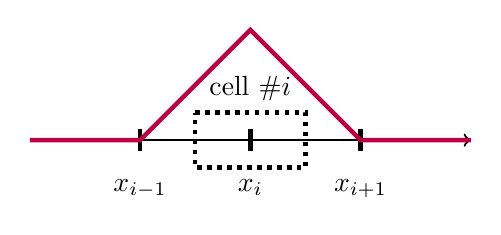
\begin{tikzpicture}[ultra thick, scale = 1.4]
    \draw[->,thick] (0,0) -- (4,0);
    \draw (1, -0.1) -- (1 , 0.1);
    \draw (2, -0.1) -- (2 , 0.1);
    \draw (3, -0.1) -- (3 , 0.1);
    \draw[purple] (0,0) -- (1,0) -- (2,1) -- (3,0) -- (4,0);
    \node[anchor = north] at (1,-0.25) {$x_{i-1}$};
    \node[anchor = north] at (2,-0.25) {$x_{i}$};
    \node[anchor = north] at (3,-0.25) {$x_{i+1}$};
    \draw[dotted] (1.5, 0.25) -- (2.5,0.25) -- (2.5, -0.25) -- (1.5, -0.25) -- cycle;
    \node[anchor = south] at (2, 0.25) {cell $\# i$};
\end{tikzpicture}
\hfill
\begin{tikzpicture}[ultra thick, scale = 1.4]
    \draw[->,thick] (0,0) -- (4,0);
    \draw (1, -0.1) -- (1 , 0.1);
    \draw (2, -0.1) -- (2 , 0.1);
    \draw (3, -0.1) -- (3 , 0.1);
    \draw[kit-purple] (0,0) -- (1,0) -- (2,1) -- (3,0) -- (4,0);
    \draw[kit-blue] (0,0) -- (1,1) -- (2,0) -- (4,0);
    \draw[kit-cyan, dotted] (0,1) -- (1,0) -- (4,0);
    \draw[kit-green, dotted] (0,0) -- (3,0) -- (4,1);
    \draw[kit-orange] (0,0) -- (2,0) -- (3,1) -- (4,0);
    \node[anchor = north] at (1,-0.25) {$x_{i-1}$};
    \node[anchor = north] at (2,-0.25) {$x_{i}$};
    \node[anchor = north] at (3,-0.25) {$x_{i+1}$};
    \node[anchor = south] at (1,1) {\textcolor{kit-blue}{$\ip_{i-1}$}};
    \node[anchor = south] at (2,1) {\textcolor{kit-purple}{$\ip_{i}$}};
    \node[anchor = south] at (3,1) {\textcolor{kit-orange}{$\ip_{i+1}$}};
    %\draw[dotted] (1.5, 0.25) -- (2.5,0.25) -- (2.5, -0.25) -- (1.5, -0.25) -- cycle;
    %\node[anchor = south] at (2, 0.25) {cell $\# i$};
\end{tikzpicture}
\caption{Linear interpolation operator. On the right $\ip_i$ on the right $\ip_{i-1}$, $\ip_{i}$, $\ip_{i+1}$.}
    \label{fig:linearInt2d}
\end{figure}
In one dimension the interpolation is only supported by two cell centers while in two dimensions we use the four surrounding nodes, see Fig \ref{fig:finter3DLinear}. 


%\Todo{Add 2d}
\begin{figure}[h!]
\label{fig:int2D}
\tdplotsetmaincoords{70}{120}
    \begin{tikzpicture}[tdplot_main_coords,line cap=butt,line join=round,c/.style={circle,fill,inner sep=1.25pt},
        declare function={a=4;h=3;}]
   % Outer square corners
  \coordinate (Z) at (-a/4, -a/4, 0);
  \coordinate (Y) at (5*a/4, -a/4, 0);
  \coordinate (X) at (5*a/4, 5*a/4, 0);
  \coordinate (W) at (-a/4, 5*a/4, 0);
  \coordinate (V) at (-a/4, a/2 ,0);
  \coordinate (U) at (a/2, 5*a/4,0);
  \coordinate (T) at (a/2, -a/4,0);
  \coordinate (R) at (5*a/4, a/2,0);

  % Outer square
  \draw[dotted] (Z) -- (Y) -- (X) -- (W) -- cycle;

  % Grid of 16 squares (4x4)
  \foreach \i in {0,1,2} {
    \foreach \j in {0,1,2} {
      %\draw[dotted](-a/4 + \i*a/2, -a/4 + \j*a/2, 0) rectangle         (-a/4 + (\i+1)*a/2, -a/4 + (\j+1)*a/2, 0);
      \pgfmathsetmacro{\xlow}{-a/4 + \i*a/2}
    \pgfmathsetmacro{\ylow}{-a/4 + \j*a/2}
    \pgfmathsetmacro{\xhigh}{-a/4 + (\i+1)*a/2}
    \pgfmathsetmacro{\yhigh}{-a/4 + (\j+1)*a/2}
    \draw[dotted] (\xlow,\ylow,0) -- (\xlow,\yhigh,0) -- (\xhigh,\yhigh,0) -- (\xhigh,\ylow,0) --cycle;
    }
  }
        \path
        (0,0,0) coordinate (A)
        (a,0,0) coordinate (B)
        (a,a,0) coordinate (C)
        (0,a,0) coordinate (D)
        (0,a/2,0) coordinate (E)
        (a/2,0,0) coordinate (F)
        (a,a/2,0) coordinate (G)
        (a/2,a,0) coordinate (H)
    (a/2,a/2,0) coordinate (O)      
    (a/2,a/2,h)  coordinate (S);
\shade[shading=axis, bottom color=kit-purple!60, top color=black!80, opacity =0.5] (S) -- (A) -- (B) -- cycle;
\shade[shading=axis, bottom color=kit-purple!60, top color=black!80, opacity =0.5] (S) -- (A) -- (D) -- cycle;
\shade[shading=axis, bottom color=kit-purple!60, top color=black!80, opacity =0.5] (S) -- (C) -- (D) -- cycle;
\shade[shading=axis, bottom color=kit-purple!60, top color=black!80, opacity =0.5] (S) -- (C) -- (B) -- cycle;
\shade[shading=axis, right color=kit-purple!60, left color=kit-purple!60, opacity=0.5]
  (Y) -- (Z) -- (A) -- (B) -- cycle;
\shade[shading=axis, bottom color=kit-purple!60, top color=kit-purple!60, shading angle=90, opacity=0.5] 
  (Y) -- (X) -- (C) -- (B) -- cycle;
\shade[shading=axis, top color=kit-purple!60, bottom color=kit-purple!60, opacity =0.5] (X) -- (W) -- (D) -- (C) -- cycle;
\shade[shading=axis, top color=kit-purple!60, bottom color=kit-purple!60, opacity =0.5] (W) -- (Z) -- (A) -- (D) -- cycle;
%\draw (S) -- (D) -- (C) -- (B) -- cycle (S) -- (C);
\draw[purple,thick] (S) -- (D);
\draw[purple,thick] (S) -- (C);
\draw[purple,thick] (S) -- (B);
\draw[purple,thick] (S) -- (G);
\draw[purple,thick] (S) -- (H);
\draw[purple,thick] (C) -- (X);
\draw[purple,thick] (A) -- (Z);
\draw[purple,thick] (B) -- (Y);
\draw[purple,thick] (D) -- (W);
%RTUV
\draw[purple,thick] (F) -- (T);
\draw[purple,thick] (E) -- (V);
\draw[purple,thick] (G) -- (R);
\draw[purple,thick] (H) -- (U);
%\draw[dashed] (S) -- (A) --(D) (A) -- (B) (S);
\draw[kit-purple,thick,dashed] (S) -- (E);
\draw[kit-purple, thick, dashed] (S) -- (F);
\draw[kit-purple,dashed,thick] (S) -- (A);


        \path foreach \p/\g/\lbl in {A/-50/x_{i-1,j-1},B/-90/x_{i-1,j+1},C/-90/x_{i+1,j+1},D/-50/x_{i+1,j-1},S/0/1,O/180/x_{i,j},E/-90/x_{i,j-1},F/-90/x_{i-1,j},G/-90/x_{i,j+1},H/-90/x_{i+1,j}}{(\p)node[c]{}+(\g:4mm) node{$\lbl$}};  
    \end{tikzpicture}
    \hfill
    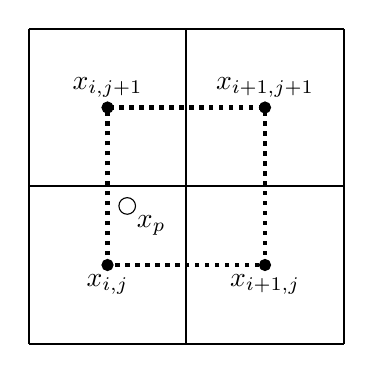
\begin{tikzpicture}[declare function={a=2;}]
        \coordinate (A) at (0,0);
        \coordinate (B) at (a,0);
        \coordinate (C) at (2*a,0);
        \coordinate (D) at (0,a);
        \coordinate (E) at (a,a);
        \coordinate (F) at (2*a,a);
        \coordinate (G) at (0,2*a);
        \coordinate (H) at (a,2*a);
        \coordinate (I) at (2*a,2*a);
        \draw[thick] (A) -- (C);
        \draw[thick] (D) -- (F);
        \draw[thick] (G) -- (I);        
        \draw[thick] (A) -- (G);
        \draw[thick] (B) -- (H);
        \draw[thick] (C) -- (I);     
        \filldraw[black] (a/2,a/2) circle (2pt) node[anchor = north]{$x_{i,j}$};
        \filldraw[black] (3*a/2,a/2) circle (2pt) node[anchor = north]{$x_{i+1,j}$};
        \filldraw[black] (a/2,3*a/2) circle (2pt) node[anchor = south]{$x_{i,j+1}$};
        \filldraw[black] (3*a/2,3*a/2) circle (2pt) node[anchor = south]{$x_{i+1,j+1}$};
        \draw (5*a/8,7*a/8) circle (3pt) node[anchor = north west]{$x_p$};
        \draw[dotted,ultra thick] (a/2,a/2) -- (a/2,3*a/2) -- (3*a/2, 3*a/2) -- (3*a/2, a/2) -- cycle;
        %\node at (a/2,a/2) {$x_{i,j}$};
    \end{tikzpicture}
    \caption{Interpolation in two dimensions. On the right all cell centers used for the interpolation of the particle, on the left a linear interpolation function for the cell center $i,j$.}
    \label{fig:finter3DLinear}
\end{figure}


% \begin{figure}[h!]
%     \begin{tikzpicture}[scale = 0.4, font = \huge]
%         \begin{axis}[
%     axis lines=left,
%     xmin=-3, xmax=3,
%     ymin=0, ymax=1,
%     domain=-3:3,
%     samples=200,
%     width=18cm,
%     height=6cm,
%     axis line style={->},
%     xtick = {-2,-1,0,1,2},
%     xticklabels={$x_{i-2}$, $x_{i-1}$,$x_i$,$x_{i+1}$,$x_{i+2}$},
%     ytick={1.0}
%     ]
%     \addplot[red, ultra thick] (-3,0) -- (-1,0) -- (0,1) -- (1,0) -- (3,0);
%     \addplot[red, ultra thick, domain=-3:-1] {0};
%     \addplot[red, ultra thick, domain=-1:0] {1-abs(x)/(1)};
%     \addplot[red, ultra thick, domain=0:1] {1-abs(x)/(1)};
%     \addplot[red, ultra thick, domain=1:3] {0};
%     \end{axis}
%     \end{tikzpicture}
%     \caption{Linear interpolation for the cell centers}
% \end{figure}
% The \MP-method uses the interpolation operator both for cell faces and for cell center interpolation.
% For cell faces the interpolation operators are shifted by half a cell.
% \begin{equation*}
%     \ifg_{i+1/2}^\x (\x_p) = \begin{cases}
%         0 & \x_{i-1/2} \geq \x_p \geq \x_{i+1/2} \\
%         1 & \x_p = \x_{i+1/2}
%     \end{cases}
% \end{equation*}
The interpolation operator satisfies
\begin{equation*}
    \sum_{\xi} \ip_\xi^\x (\x_p) =1 \qquad \forall particles, cells
\end{equation*}
when summing over all Eulerian cells this holds for $\ip$.
For the linear case this can be observed in the sketch above.

In the two dimensional case the grid properties are mapped to the particle by using the four enclosing cell centers, see figure \ref{fig:finter3DLinear}. 
Interpolating a quantity $Q$ from the Eulerian grid to the particle position we use
\begin{equation*}
    Q_p = \ip_{i,j} (\xp) Q_{i,j} + \ip_{i+1,j} (\xp) Q_{i+1,j}+ \ip_{i,j+1} (\xp) Q_{i,j+1}+ \ip_{i+1,j+1} (\xp) Q_{i+1,j+1}
\end{equation*}
with the two dimensional interpolation operator being formed by the product of the two one dimensional operators
\begin{equation*}
    \ip_{i,j} = \ip_i^\x \ip_j^y.
\end{equation*}


Analogously, in three dimensions we have
\begin{equation*}
    \ip_{i,j,k} = \ip^x_i \ip^y_j \ip^z_k,
\end{equation*}
with the operators $\ip^y$ and $\ip^z$ analogue to $\ip^z$ and the interpolation of grid quantities is
\begin{equation*}
    \gp_p = \ip_\xi ( \xp) \gp_\xi.
\end{equation*}

\begin{equation}
    \label{eq:svf}
    \pvf = \MultiIntegral{2} \pd \dfrac{\m}{\rp} d \m d \up.
\end{equation}

For example the discrete particle volume fraction is defined via the interpolation
\begin{equation*}
    \pvf_{p_{i,j,k}} = \dfrac{1}{V_{i,j,k}} \sum_{\kappa } N_{p,\kappa} V_{p_{i,j,k}} \ip_{i,j,k} (\x_{p_\kappa}),
\end{equation*}
with the particle volume $V$.
The product of interpolation operators for a grid property $\gp$ where the property is mapped to a particle location and the to the grid is defined as
\begin{equation*}
    \ip_\zeta (\xp) \sum_{\xi}^8 \ip_\xi (\xp) \gp_\xi = \sum_{\xi}^{8} \ip_\zeta.
\end{equation*}
The product of two interpolation operators for cells is defined as
\begin{equation}
\label{eq:ipOrtho}
    \ip_\zeta(\boldsymbol{\x}_{p_{\kappa}})\ip_{\xi} (\boldsymbol{x}_{p_\iota}) = \begin{cases}
        \ip_{\xi}(\boldsymbol{x}_{p_\kappa}) & \text{if } \xi = \zeta \text{ and } \iota = \kappa \\
        0 & \text{else}.
    \end{cases}
\end{equation} 

% as well as the gradient
% \begin{equation*}
%     \nabla \gp_p = \sum_{\xi =1}^{N} \nabla \ip_\xi (\xp) \gp_\xi + \sum_{\xi =1}^{N} \ip_\xi ( \xp) (\nabla \gp)_{\xi}.
% \end{equation*}
For the one dimensional case we can calculate the spatial derivative of the linear interpolation operator with the help of the cell-face interpolation function. For an equidistant grid we have a top hat function
\begin{equation*}
    \ifg_{i+1/2} = \begin{cases}
        1 & \text{if }   \x_i \leq \x_p < \x_{i+1} \\
        0 & \text{if }   \x_p < \x_{i} \text{ or } \x \geq \x_{i+1},
    \end{cases} \qquad \hspace{1cm}
    \label{eq:gradInterp}
    \dfrac{\partial \ip_i}{\partial \x} = \dfrac{1}{\Delta \x} ( \ifg_{i-1/2} - \ifg_{i+1/2})
\end{equation*}
that is depicted in \ref{fig:topHat}.
\begin{figure}[h!]
    \centering
    \begin{subfigure}[b]{0.45 \linewidth}
    \begin{tikzpicture}[thick, scale = 1.4]
    \draw[->] (0,0) -- (4,0);
    \draw (1, -0.1) -- (1 , 0.1);
    \draw (2, -0.1) -- (2 , 0.1);
    \draw (3, -0.1) -- (3 , 0.1);
    \draw[kit-red,ultra thick] (0,0) -- (1,0) -- (1,1) -- (2,1) -- (2,0) -- (4,0);
    \draw[kit-blue,ultra thick,dashed] (0,0) -- (2,0) -- (2,1) -- (3,1) -- (3,0) -- (4,0);
    \node[anchor = north] at (1,-0.25) {$x_{i-1}$};
    \node[anchor = north] at (2,-0.25) {$x_{i}$};
    \node[anchor = north] at (3,-0.25) {$x_{i+1}$};
    \draw[dotted] (1.5, 1.25) -- (2.5,1.25) -- (2.5, -0.75) -- (1.5, -0.75) -- cycle;
    \node[anchor = south,kit-red] at (0.5, 0.5) {$T_{i-1/2}$};
    \node[anchor = south,kit-blue] at (3.5,0.5) {$T_{i+1/2}$};
    \node[anchor = south] at (2, 1.25) {cell $\# i$};
\end{tikzpicture}
    \label{fig:placeholder}
    \caption{Top hat function for the the cell faces $i-\frac{1}{2}$ (red) and $i+\frac{1}{2}$ (blue).}
    \end{subfigure}
    \hfill
    \begin{subfigure}[b]{0.45 \linewidth}
    \centering
    \begin{tikzpicture}[thick, scale = 1.4]
    \draw[->] (0,0) -- (4,0);
    \draw (1, -0.1) -- (1 , 0.1);
    \draw (2, -0.1) -- (2 , 0.1);
    \draw (3, -0.1) -- (3 , 0.1);
    \draw[kit-red, ultra thick] (0,0) -- (1,0) -- (2,1) -- (3,0) -- (4,0);
    \draw[kit-blue,dashed,ultra thick] (0,0) -- (1,0);
    \draw[kit-blue,dashed, ultra thick] (1,1) -- (2,1);
    \draw[kit-blue,dashed, ultra thick](2,-1) -- (3,-1);
    \draw[kit-blue, dashed, ultra thick] (3,0) -- (4,0);
    \node[anchor = north] at (1,-0.15) {$x_{i-1}$};
    \node[anchor = north] at (2,-0.15) {$x_{i}$};
    \node[anchor = north] at (3,-0.15) {$x_{i+1}$};
    %\draw[dotted] (1.5, 0.25) -- (2.5,0.25) -- (2.5, -0.25) -- (1.5, -0.25) -- cycle;
    %\node[anchor = south] at (2, 0.25) {cell $\# i$};
\end{tikzpicture}
\caption{Interpolation operator $\ip_i$ in purple and its gradient in blue. For illustration purposes the grid has a spacing of $\Delta x = 1$.}
\end{subfigure}
\caption{Top hat function and linear interpolation with gradient.}
\label{fig:topHat}
\end{figure}

The choice of values for the interpolation of cell face values depicted in Fig. \ref{fig:2dintall} in two dimensions is not quite as obvious as in one dimension. In Fig. \ref{fig:intTwoNeigh} and Fig. \ref{fig:bilinearInt}  two different options are presented.
% In two dimensions we need to choose the cell faces we want to use for the interpolation. In figure \ref{fig:2dintall} we can see the velocities at the cell face centers which we will use in the following. 

\begin{figure}[h!]
    \centering
    \begin{subfigure}[t]{0.4\textwidth}
    \begin{tikzpicture}[declare function={a=2.5;}]
        \coordinate (A) at (0,0);
        \coordinate (B) at (a,0);
        \coordinate (C) at (2*a,0);
        \coordinate (D) at (0,a);
        \coordinate (E) at (a,a);
        \coordinate (F) at (2*a,a);
        \coordinate (G) at (0,2*a);
        \coordinate (H) at (a,2*a);
        \coordinate (I) at (2*a,2*a);
        \draw[thick] (A) -- (C);
        \draw[thick] (D) -- (F);
        \draw[thick] (G) -- (I);        
        \draw[thick] (A) -- (G);
        \draw[thick] (B) -- (H);
        \draw[thick] (C) -- (I);     
        \filldraw[black] (a/2,a/2) circle (2pt) node[anchor = north]{$x_{i,j}$};
        \filldraw[black] (3*a/2,a/2) circle (2pt) node[anchor = north]{$x_{i+1,j}$};
        \filldraw[black] (a/2,3*a/2) circle (2pt) node[anchor = north]{$x_{i,j+1}$};
        \filldraw[black] (3*a/2,3*a/2) circle (2pt) node[anchor = north]{$x_{i+1,j+1}$};
        \draw (10*a/8,7*a/8) circle (3pt) node[anchor = north west]{$x_p$};
        \draw[->,ultra thick,kit-purple] (-a/4,a/2) -- node[above] {$u_{i-1/2,j}$}(a/4, a/2);
        \draw[->,ultra thick,kit-purple] (3*a/4,a/2) --node[above] {$u_{i+1/2,j}$} (5*a/4, a/2);
        \draw[->,ultra thick,kit-purple] (7*a/4,a/2) -- node[above] {$u_{i+3/2,j}$}(9*a/4, a/2);
        \draw[->,ultra thick,kit-purple] (a/4,a) -- node[above] {$u_{i,j+1/2}$}(3*a/4, a);
        \draw[->,ultra thick,kit-purple] (5*a/4,a) -- node[above] {$u_{i,j+3/2}$}(7*a/4, a);
        \draw[->,ultra thick,kit-purple] (-a/4,3*a/2) -- node[above] {$u_{i-1/2,j+1}$}(a/4, 3*a/2);
        \draw[->,ultra thick,kit-purple] (3*a/4,3*a/2) -- node[above] {$u_{i+1/2,j+1}$}(5*a/4, 3*a/2);
        \draw[->,ultra thick,kit-purple] (7*a/4,3*a/2) --node[above] {$u_{i+1/2,j+1}$} (9*a/4, 3*a/2);
        \draw[->,ultra thick,kit-purple] (a/4,0) -- node[above] {$u_{i,j+1/2}$}(3*a/4, 0);
        \draw[->,ultra thick,kit-purple] (5*a/4,0) -- node[above] {$u_{i+1,j-1/2}$}(7*a/4, 0);
        \draw[->,ultra thick,kit-purple] (a/4,2*a) -- node[below] {$u_{i+1,j+1/2}$}(3*a/4, 2*a);
        %\draw[arrow] (pro1) -- node[right] {After convergence} (pro2);
        \draw[->,ultra thick,kit-purple] (5*a/4,2*a) --node[below] {$u_{i+1,j+3/2}$} (7*a/4, 2*a);
        %\node at (a/2,a/2) {$x_{i,j}$};
    \end{tikzpicture}
     \caption{Velocity at cell faces in $x$-direction used for interpolation.}
     \label{fig:2dintall}
    \end{subfigure}
    \hfill
    \begin{subfigure}[t]{0.4\textwidth}
    \begin{tikzpicture}[declare function={a=2.5;}]
        \coordinate (A) at (0,0);
        \coordinate (B) at (a,0);
        \coordinate (C) at (2*a,0);
        \coordinate (D) at (0,a);
        \coordinate (E) at (a,a);
        \coordinate (F) at (2*a,a);
        \coordinate (G) at (0,2*a);
        \coordinate (H) at (a,2*a);
        \coordinate (I) at (2*a,2*a);
        \draw[thick] (A) -- (C);
        \draw[thick] (D) -- (F);
        \draw[thick] (G) -- (I);        
        \draw[thick] (A) -- (G);
        \draw[thick] (B) -- (H);
        \draw[thick] (C) -- (I);     
        \filldraw[black] (a/2,a/2) circle (2pt) node[anchor = north east]{$x_{i,j}$};
        \filldraw[black] (3*a/2,a/2) circle (2pt) node[anchor = north west]{$x_{i+1,j}$};
        \filldraw[black] (a/2,3*a/2) circle (2pt) node[anchor = south east]{$x_{i,j+1}$};
        \filldraw[black] (3*a/2,3*a/2) circle (2pt) node[anchor = south west]{$x_{i+1,j+1}$};
        \draw (10*a/8,6*a/8) circle (3pt) node[anchor = south east]{$x_p$};
        % \draw[->,ultra thick,purple] (-a/4,a/2) -- node[above] {$u_{i-1/2,j}$}(a/4, a/2);
        \draw[->,ultra thick,kit-purple] (3*a/4,a/2) --node[above] {$u_{i+1/2,j}$} (5*a/4, a/2);
        % \draw[->,ultra thick,purple] (7*a/4,a/2) -- node[above] {$u_{i+3/2,j}$}(9*a/4, a/2);
        % \draw[->,ultra thick,purple] (a/4,a) -- node[above] {$u_{i,j+1/2}$}(3*a/4, a);
        % \draw[->,ultra thick,purple] (5*a/4,a) -- node[above] {$u_{i,j+3/2}$}(7*a/4, a);
        % \draw[->,ultra thick,purple] (-a/4,3*a/2) -- node[above] {$u_{i-1/2,j+1}$}(a/4, 3*a/2);
        \draw[->,ultra thick,kit-purple] (3*a/4,3*a/2) -- node[above] {$u_{i+1/2,j+1}$}(5*a/4, 3*a/2);
        % \draw[->,ultra thick,purple] (7*a/4,3*a/2) --node[above] {$u_{i+1/2,j+1}$} (9*a/4, 3*a/2);
        % \draw[->,ultra thick,purple] (a/4,0) -- node[above] {$u_{i,j+1/2}$}(3*a/4, 0);
        % \draw[->,ultra thick,purple] (5*a/4,0) -- node[above] {$u_{i+1,j-1/2}$}(7*a/4, 0);
        % \draw[->,ultra thick,purple] (a/4,2*a) -- node[above] {$u_{i+1,j+1/2}$}(3*a/4, 2*a);
        % %\draw[arrow] (pro1) -- node[right] {After convergence} (pro2);
        % \draw[->,ultra thick,purple] (5*a/4,2*a) --node[above] {$u_{i+1,j+3/2}$} (7*a/4, 2*a);
        \draw[->, ultra thick, kit-purple] ( a/2,3*a/4) -- node[above left] {$v_{i/2,j+1/2}$} (a/2,5*a/4);
        \draw[->, ultra thick, kit-purple] ( 3*a/2,3*a/4) -- node[above right] {$v_{i+1,j+1/2}$} (3*a/2,5*a/4);
        %\node at (a/2,a/2) {$x_{i,j}$};
        \draw[ultra thick, dashed, kit-purple] (a/2,a/2) -- (3*a/2,a/2) -- (3*a/2,3*a/2) -- (a/2,3*a/2) -- cycle;
    \end{tikzpicture}
    \caption{Velocity values used in the closest-neighbor interpolation method for interpolating from the Eulerian grid to $\xp$.}
    \label{fig:intTwoNeigh}
    \end{subfigure}

    
    \begin{subfigure}[b]{0.4\textwidth}
    \begin{tikzpicture}[declare function={a=2.5;}]
        \coordinate (A) at (0,0);
        \coordinate (B) at (a,0);
        \coordinate (C) at (2*a,0);
        \coordinate (D) at (0,a);
        \coordinate (E) at (a,a);
        \coordinate (F) at (2*a,a);
        \coordinate (G) at (0,2*a);
        \coordinate (H) at (a,2*a);
        \coordinate (I) at (2*a,2*a);
        \draw[thick] (A) -- (C);
        \draw[thick] (D) -- (F);
        \draw[thick] (G) -- (I);        
        \draw[thick] (A) -- (G);
        \draw[thick] (B) -- (H);
        \draw[thick] (C) -- (I);     
        \filldraw[black] (a/2,a/2) circle (2pt) node[anchor = north west]{$x_{i,j}$};
        \filldraw[black] (3*a/2,a/2) circle (2pt) node[anchor = north east]{$x_{i+1,j}$};
        \filldraw[black] (a/2,3*a/2) circle (2pt) node[anchor = north]{$x_{i,j+1}$};
        \filldraw[black] (3*a/2,3*a/2) circle (2pt) node[anchor = north]{$x_{i+1,j+1}$};
        % \draw[->,ultra thick,purple] (-a/4,a/2) -- node[above] {$u_{i-1/2,j}$}(a/4, a/2);
        
        %\draw[->,ultra thick,purple] (a/4,0) -- node[above] {$u_{i,j+1/2}$}(3*a/4, 0);
        %\draw[->,ultra thick,purple] (5*a/4,0) -- node[above] {$u_{i+1,j-1/2}$}(7*a/4, 0);
        %\draw[->,ultra thick,purple] (a/4,2*a) -- node[above] {$u_{i+1,j+1/2}$}(3*a/4, 2*a);
        %\draw[arrow] (pro1) -- node[right] {After convergence} (pro2);
        %\draw[->,ultra thick,purple] (5*a/4,2*a) --node[above] {$u_{i+1,j+3/2}$} (7*a/4, 2*a);
        \shade[shading=axis, top color=kit-purple!60, bottom color=purple!60, opacity =0.5] (a,a/2) -- (a,3*a/2) -- (2*a,3*a/2) -- (2*a,a/2) -- cycle;
        \draw[ultra thick,dashed, kit-purple](a,a/2) -- (a,3*a/2) -- (2*a,3*a/2) -- (2*a,a/2) -- cycle;
        \shade[shading=axis, top color=kit-blue!40, bottom color=blue!40, opacity =0.5] (a/2,0) -- (3*a/2,0) -- (3*a/2,a) -- (a/2,a) -- cycle;
        \draw[ultra thick,dashed, kit-blue](a/2,0) -- (3*a/2,0) -- (3*a/2,a) -- (a/2,a) -- cycle;
        \draw[->,ultra thick,kit-purple] (3*a/4,a/2) --node[above] {$u_{i+1/2,j}$} (5*a/4, a/2);
        \draw[->,ultra thick,kit-purple] (7*a/4,a/2) -- node[above] {$u_{i+3/2,j}$}(9*a/4, a/2);
        %\draw[->,ultra thick,purple] (a/4,a) -- node[above] {$u_{i,j+1/2}$}(3*a/4, a);
        %\draw[->,ultra thick,purple] (5*a/4,a) -- node[above] {$u_{i,j+3/2}$}(7*a/4, a);
        %\draw[->,ultra thick,purple] (-a/4,3*a/2) -- node[above] {$u_{i-1/2,j+1}$}(a/4, 3*a/2);
        \draw[->,ultra thick,kit-purple] (3*a/4,3*a/2) -- node[above] {$u_{i+1/2,j+1}$}(5*a/4, 3*a/2);
        \draw[->,ultra thick,kit-purple] (7*a/4,3*a/2) --node[above] {$u_{i+3/2,j+1}$} (9*a/4, 3*a/2);
        \draw[->,ultra thick, kit-blue] (a/2,3*a/4) -- node[below left] {$v_{i,j+1/2}$}(a/2,5*a/4);
        \draw[->,ultra thick, kit-blue] (3*a/2,-a/4) -- node[below right] {$v_{i+1,j-1/2}$}(3*a/2,a/4);
        \draw[->,ultra thick, kit-blue] (a/2,-a/4) -- node[above left]{$v_{i,j-1/2}$} (a/2,a/4);
        \draw[->,ultra thick, kit-blue] (3*a/2,3*a/4) -- node[below right] {$v_{i+1, j+1/2}$} (3*a/2,5*a/4);
        \draw (10*a/8,7*a/8) circle (3pt) node[anchor = north west]{$x_p$};
        %\node at (a/2,a/2) {$x_{i,j}$};
    \end{tikzpicture}
     \caption{Velocity values used in the bilinear interpolation, adapted from \cite{MP2d}.}
     \label{fig:bilinearInt}
    \end{subfigure}
    %\caption{Interpolation with face values.}
\end{figure}
Once again we use the top hat functions we defined earlier.
For the two-neighbor interpolation we use the velocity $u$ in $\x$ direction and the velocity $v$ in $y$ direction. As the name suggests we use the two neighboring velocities, see figure ~\ref{fig:intTwoNeigh}. We use two top hat functions for the $\x$-face velocity
\begin{align}
    \ip_{i+1/2,j}^{T} &= \ifg_{i+1/2} \ifg_j \\
    \u_{g,p} &= \ip_{i+1/2,j}^{T} (\xp) \u_{i+1/2,j} +  \ip_{i+1/2,j+1}^{TS} (\xp) \u_{i+1/2,j+1} \\
    v_{g,p} &= \ip_{i,j+1/2}^{T} (\xp) \u_{i,j+1/2} +  \ip_{i+1,j+1/2}^{TS} (\xp) \u_{i+1,j+1/2}.
\end{align}

The second option is to use face bilinear interpolation as shown in figure \subref{fig:bilinearInt}. Compared to the closest neighbor interpolation we now double the cell faces used to four per direction. 
For both the $x$ and the $y$ direction we use the encompassing faces for the interpolation operators
\begin{equation*}
    \ip_{i+1/2,j}^S = \ip^x_{i+1/2} \ip^y_{j} \qquad \ip_{i,j+1/2}^S = \ip^x_i \ip^y_{j+1/2}
\end{equation*}
and then have the interpolated velocity
\begin{align*}
    \u_{g,p} = \ip^S_{i+1/2,j} (\xp) \u_{i+1/2,j} + \ip_{i+3/2,j}^S (\xp) \u_{i+3/2,j} + \ip_{i+3/2,j+1}^S (\xp) \u_{i+3/2,j+1} + \ip^S_{i+1/2,j+1}(\xp)\u_{i+1/2,j+1}\\
    v_{g,p} =  \ip^S_{i,j+1/2} (\xp) v_{i,j+1/2} + \ip^S_{i+1,j+1/2} (\xp) v_{i+1,j+1/2} + \ip^S_{i+1,j-1/2} (\xp) v_{i+1,j-1/2}+\ip^S_{i,j-1/2} (\xp) v_{i,j-1/2}.
\end{align*}
%\color{gray}
%\Todo{Which one is used?}

For the momentum continuity equation, we also need the gradient of the interpolation operator.
The grid property $\gp$ mapped to the particle location $\xp$ is
\begin{equation*}
    \nabla \gp_p = \sum_{\xi =1}^{N} \nabla \ip_{\xi}(\xp) \gp_{\xi} + \sum_{\xi = 1}^N \ip_{\xi} ( \xp) (\nabla \gp)_\xi = \sum_{\xi =1}^N \ip_{\xi} ( \xp) (\nabla \gp)_\xi.
\end{equation*}
Here the particle position is fixed leading to the second equality.
Furthermore can also map the gradient of a grid property $\gp$ to and from the particle
\begin{equation*}
    \nabla \ip_\zeta (\xp) \cdot \sum_{\xi =1}^8 \ip_\xi ( \xp ) \nabla \gp_\xi = \sum_{i=1}^8 \nabla \ip_\zeta ( \xp ) \cdot [\ip_\xi (\xp) \nabla \gp_\xi].
\end{equation*}
To simplify the equation we first look a the product of an interpolation operator with the gradient of an interpolation operator
\begin{equation*}
    \sum_\xi \ip_\xi \nabla \ip_\zeta = \sum_\xi \ip_{x_\zeta} \ip_{y_\zeta} \ip_{z_\zeta} \begin{pmatrix}
        \frac{\partial \ip_{x_\xi}}{\partial x} \ip_{y_\xi} \ip_{z_\xi} \\
        \frac{\partial \ip_{y_\xi}}{\partial y} \ip_{x_\xi} \ip_{z_\xi} \\
        \frac{\partial \ip_{z_\xi}}{\partial z} \ip_{x_\xi} \ip_{y_\xi}
    \end{pmatrix}.
\end{equation*}
We can apply the orthogonality property from equation \eqref{eq:ipOrtho} and then receive
\begin{equation*}
    \nabla \ip_\zeta ( \xp ) \cdot \sum_{\xi=1}^8 \ip_\xi ( \xp ) \nabla \gp_\xi = \ip_\zeta \left[ \dfrac{\partial \ip_{x_\zeta}}{\partial x} \boldsymbol{e}_x + \dfrac{\partial \ip_{y_\zeta}}{\partial y} \boldsymbol{e}_y + \dfrac{\partial \ip_{z_\zeta}}{\partial z} \boldsymbol{e}_z\right].
\end{equation*}
We will look more specifically at the interpolation used in \OF later in \ref{sec:OFInterpolation}.


\subsection{Numerical Solution without damping terms}
The interpolation operators introduced in the previous section are used in the \MP method to map particle properties between the Eulerian grid and the particle positions.
The method can be roughly split into the the following three steps in each time step.
First the method calculates the provisional particle positions based on the previous velocity and particle positions.
These positions are used to map the properties like particle volume fraction to the Eulerian grid.
Then the momentum and continuity equation are solved on the Eulerian map.
Derivative terms for example for the solid stress are mapped back to the particles and used to calculate the advanced particle positions.
This completes the completes the time step.
In the following we will derive each step and look at the implicit approximations used.

For the numerical solution we use the parcels mentioned above. As per the assumption made in equation \eqref{eq:partConservation}, the number of particles in a volume is conserved in particle phase space. 
Therefore the parcels have a constant number of particles.
We assume that a particle's mass and volume is constant.
Advanced particle positions are then calculated by
\begin{equation}
    \label{eq:MPposition}
    \xp^{n+1} = \xp^{n} + \Delta t \up^{n+1}, \ n \in \mathbb{N} \qquad \xp^{0} = \x_0
\end{equation}
and the velocity is rearranging by the discretized acceleration \eqref{eq:accel}
% \Todo{Anpassen auf altes Paper}
\begin{align}
    \dfrac{\up^{n+1} - \up^{n}}{\Delta \tvar} &= \d (\upi^{n+1} -
    \up^{n+1})  - \dfrac{1}{\rp} \nabla \p_p^{n+1} - \dfrac{1}{\rp \pvf} \nabla \scs^{n+1} - \g  \nonumber \\
    \Leftrightarrow \up^{n+1} &= \dfrac{\up^n + \Delta \tvar \left[ \d S\up^{n+1} - \dfrac{1}{\rp} \nabla \p_p^{n+1} - \dfrac{1}{\rp \pvf} \nabla \scs^{n+1} - \g \right]}{1 + \Delta \tvar \d} .\label{eq:errVel} 
\end{align}

In the following we will restrict ourselves to the one dimensional case for easier reading. 
For the gradients we use a differential quotient 
\begin{equation}
\label{eq:MPvelocity}
    \up^{n+1} = \dfrac{\up^n + \Delta \tvar \left[\d \tilde{u_{p}} - \g - \dfrac{1}{\rp} \left(\dfrac{\tilde{\p}_{i+1} - \tilde{\p}_i}{\Delta \x} \right)_p - \dfrac{1}{\rp \pvf} \left( \dfrac{\tilde{\ss}_{i+1} - \tilde{\ss}_i}{\Delta \x}\right)_p \right]}{1 + \Delta \tvar \d}
\end{equation}
Variables marked with a tilde $\tilde{\cdot}$ are implicit approximations to the advanced-time step. They as well as the interphase momentum transfer will be defined in the following.

The equations for updating the position \eqref{eq:MPposition} and velocity \eqref{eq:MPvelocity} are used at the end of a time step to calculate the new particle velocities and positions.
These two equations are the first of eight equations.
In total we will need eight equations which we will derive in the following.
We start by applying a central diffrencing scheme to the fluid continuity equation
\begin{equation}
    \label{eq:gasContDisc}
    \dfrac{(\fvf \rf)_i^{n+1} - (\fvf \rf)_i^n}{\Delta \tvar} + \dfrac{(\fvf \rf \uf)_{i+\frac{1}{2}}^{n+1}- (\fvf \rf \uf)_{i-\frac{1}{2}}^{n+1}}{\Delta \xp} = 0,
\end{equation}
and the momentum equation
\begin{equation}
    \label{eq:discMom}
    \dfrac{(\fvf \rf \uf)_{i+\frac{1}{2}}^{n+1}- (\fvf \rf \uf)_{i+\frac{1}{2}}^{n}}{\Delta \tvar} + \dfrac{(\fvf \rf \uf^2)^n_{i+1}-(\fvf \rf \uf^2)^n_{i}}{\Delta \xp} + \dfrac{\tilde{\p}_{i+1}-\tilde{p}_i}{\Delta \xp} = - \F_{i+\frac{1}{2}}-\dfrac{((\fvf \rf)_i^n + (\fvf \rf)_{i+1}^n)\g}{2}.
\end{equation}
% \Todo{Does this actually make sense?}
A different approach, a finite volume method, is use in \OF. For now though we will stick to the finite differencing scheme used in the original paper.

To approximate the convective flux $\fvf \rf \uf^2$ we it into the mass flux and the fluid velocity.
Since the mass flux is only known at the cell faces we use a central approximation scheme for the cell center. 
For the velocity, we use an upwind approximation scheme

\begin{align*}
    (\fvf \rf \uf^2)_i^n = \dfrac{\dot{\m}_{i+\frac{1}{2}}+\dot{\m}_{i-\frac{1}{2}}}{2} \cdot
    \begin{cases}
        (\uf)^n_{i- \frac{1}{2}} & \text{if } \dot{\m}_{i-\frac{1}{2}} + \dot{\m}_{i+\frac{1}{2}} > 0 \\
        (\uf)^n_{i+ \frac{1}{2}} & \text{if } \dot{\m}_{i-\frac{1}{2}} + \dot{\m}_{i+\frac{1}{2}} < 0
    \end{cases}
\end{align*}

with the mass flux calculated at the matching face and the fluid velocity calculated with the neighboring volume fraction times the fluid density
\begin{align*}
    \dot{\m}_{i+\frac{1}{2}} = (\fvf \rf \uf)^n_{i+\frac{1}{2}} \qquad (\uf)_{i+\frac{1}{2}}^n = \dfrac{2 (\fvf \rf \uf)_{i+\frac{1}{2}}}{(\fvf \rf)_{i} + (\fvf \rf)_{i+1}^n}.
\end{align*}


For the pressure we use the ideal gas assumption from above \eqref{eq:gasDensReal} that fluid pressure and the density are related we have
\begin{equation}
    \p = c_1 \rf^\gamma = c_1 \left( \dfrac{R}{\fvf}\right)^\gamma = c_1 \left( \dfrac{R}{1 - \pvf}\right)^\gamma \quad \text{with} \quad R \coloneq \fvf \rf.
\end{equation}
Because the pressure is nonlinear we use an implicit approximation to the gas pressure. 
A first order Taylor expansion around $((\fvf \rf)^{n},\pvf^n)$  evaluated at time-step $n+1$ yields
\begin{equation}
\label{eq:pTaylor}
    \p^{n+1} = \p^n + \dfrac{\partial \p}{\partial (\fvf \rf)}\bigg|^n \left[ (\fvf \rf )^{n+1} - (\fvf \rf)^n \right] +\dfrac{\partial \p}{\partial \pvf}\bigg|^n \left[ \pvf  ^{n+1} - \pvf^n \right].
\end{equation}
Both derivatives can be explicitly calculated by
\begin{equation*}
    \dfrac{\partial \p}{\partial (\fvf \rf)} = \dfrac{\partial \p}{\partial R} = c_1 \gamma \left( \dfrac{R}{\fvf}\right)^{\gamma -1} \dfrac{1}{\fvf}= \dfrac{\gamma}{R} \p
\end{equation*}
and
\begin{equation*}
    \dfrac{\partial \p}{\partial \pvf} = c_1 \gamma \dfrac{1}{1- \pvf} \left( \dfrac{R}{1 - \pvf}\right)^\gamma = \dfrac{\gamma}{1-\pvf} \p.
\end{equation*}
Inserting both back into the Taylor expansion \eqref{eq:pTaylor}
\begin{equation}
    \p_i^{n+1} = \p^n \left( 1 + \gamma \left[\dfrac{(\fvf \rf)^{n+1} - (\fvf \rf)^{n}}{(\fvf \rf)^n} + \dfrac{\widetilde{\pvf} - \pvf^n}{1 - \pvf^n} \right] \right)
\end{equation}
with $\p_i^{n}$ approximated by
\begin{equation*}
    c_1 \coloneq \dfrac{\p_{ref}}{\rgref^\gamma} \quad  \Rightarrow \quad \p_i^n = \p_{ref} \left[ \dfrac{(\fvf \rf )_i^n}{(1- \pvfi^n)\rgref} \right]^\gamma.
\end{equation*}
with $\p_{ref}$ and $\rgref$ at some reference state. For $\pvfi^n$ we use the discretization
\begin{equation*}
    \pvfi^n = \dfrac{1}{\Delta x} \sum_p \ip_i(\x_p^n) \dfrac{\m_p}{\rp} \Np.
\end{equation*}
$\pvf^{n+1}$ is approximated by $\widetilde{\pvf}$ and will be discussed later. 
%\Todo{Wandeffekte?}

For mapping properties defined at the faces back to the parcels, we define the provisional parcel position
\begin{equation}
    \label{eq:provPartPos}
    \xpp = \xp^n + \up^n \Delta \tvar.
\end{equation}
and use the cell-face interpolation function e.g.
\begin{equation}
    \label{eq:cellFaceInterpolation}
    \left( \dfrac{\tilde{\p_{i+1}} - \tilde{\p_{i}}}{\Delta x} \right)_p = \sum_i \ifg_{i+ \frac{1}{2}} (\xpp ) \frac{\tilde{p}_{i+1} - \tilde{p}_i}{\Delta x}.
\end{equation}
The solid stress is highly nonlinear. Using the old velocity and fluid properties when particles are near close pack can push particles into already close-packed space.
For the approximation of the advanced-time solids stress we again use a linearly implicit approximation, the Taylor expansion applied to \eqref{eq:solidStress} around $\pvfi^n$ evaluated at $\tilde{\pvfi}$
\begin{align}
    \ss_i^{n+1} &= \ss_i^n + \dfrac{\partial \ss}{\partial \pvf}\bigg|_n  (\pvfi^{n+1} - \pvfi^n)  \qquad \dfrac{\partial \ss}{\partial \pvf}\bigg|_n = P_s \dfrac{\pvfcp}{\pvf^2} \left( \dfrac{\pvfcp}{\pvf} -1 \right)^{-2}\\
    \Rightarrow \tilde{\ss}_i &= \ss_i^n + P_s\dfrac{\pvfcp}{(\pvfcp - \pvf)^2} (\tilde{\pvf}- \pvfi^n).
\end{align}
To approximate the volume fraction for the provisional parcel positions we first need to get it at the cell faces before we can interpolate it to the parcels. 
For cell faces we use properties from the Eulerian grid
\begin{equation}
    \label{eq:interpolationPVFCellFace}
    \pvf_{i+ \frac{1}{2}} = \dfrac{1}{\Delta x} \sum_p \ifg_{i+\frac{1}{2}} (\xpp ) \Np \dfrac{\m_p}{\rp}
\end{equation}
and then weight the volume fraction by the interpolation function to get the volume fraction at the provisional parcel position
\begin{equation}
    \label{eq:interpolatePPP}
    \pvfp = \sum_i \ifg_{i+\frac{1}{2}} (\xpp) \pvf_{i+\frac{1}{2}}.
\end{equation}

To verify the discretizations above, we look at whether the parcel momentum is conserved. 
We multiply the discretized momentum equation \eqref{eq:discMom} by $\Np \mp$  and sum over all parcels
\begin{align*}
    \sum_p \Np \mp \dfrac{\up^{n+1}-\up^n}{\Delta \tvar} =& - \sum_p \Np \mp \g - \sum_p \dfrac{\Np \mp}{\rp} \left( \dfrac{\tilde{\p}_{i+1}- \tilde{\p}_i}{\Delta \x}\right)_p + \sum_p D_p \Np \mp (\tilde{\ugp} - \up^{n+1}) \\
    &- \sum_p \dfrac{\Np \mp}{\rp \pvfp} \left( \dfrac{\tilde{\ss}_{i+1}-\tilde{\ss}_i}{\Delta \x}\right)_p.
\end{align*}
Using the previous definitions the last term becomes
\begin{align*}
    \sum_p \dfrac{\Np \mp}{\rp \pvf} \left( \dfrac{\tilde{\ss}_{i+1}-\tilde{\ss}_i}{\Delta \x}\right)_p \stackrel{\eqref{eq:cellFaceInterpolation}}{=} \sum_p \dfrac{\Np \mp}{\rp \pvf} \sum_i \ifg_{i+\frac{1}{2}}(\xpp) \dfrac{\tilde{\ss}_{i+1}-\tilde{\ss_i}}{\Delta \x} = \sum_i \sum_p \left( \dfrac{\Np \mp}{\rp} \ifg_{i+\frac{1}{2}} ( \xpp)\right)\dfrac{\tilde{\ss}_{i+1}- \tilde{\ss}_i}{\pvf_{i+\frac{1}{2}} \Delta \x}.
\end{align*}
For the last step we used
\begin{equation*}
    \pvf \stackrel{\eqref{eq:interpolatePPP}}{=} \sum_{i}  \ifg_{i+\frac{1}{2}} (\xpp) \pvf_{i+\frac{1}{2}} = \pvf_{i+\frac{1}{2}} \qquad \iff \qquad \ifg_{i+\frac{1}{2}} (\xpp) = 1
\end{equation*}
Using \eqref{eq:interpolationPVFCellFace} gives us
\begin{align*}
    \sum_i \sum_p \left( \dfrac{\Np \mp}{\rp} \ifg_{i+\frac{1}{2}} ( \xpp)\right)\dfrac{\tilde{\ss}_{i+1}- \tilde{\ss}_i}{\frac{1}{\Delta \x}\sum_p \dfrac{\Np \mp}{\rp} \ifg_{i+\frac{1}{2}} ( \xpp) \Delta \x} %= \sum_i \tilde{\ss}_{i+1}-\tilde{\ss}_i 
    = \sum_{i=0}^{N} \tilde{\ss}_{i+1} - \tilde{\ss}_i = \tilde{\ss}_N - \tilde{\ss}_0,
\end{align*}
which are the boundary sources thus proving momentum conservation.
Here we only look at the one dimensional case but this can be extended to two and three-dimensional cases with their respective boundary terms. Thus the implicit approximation conserves the momentum.

Similarly, for the advanced-time gas velocity, we use the interpolation to the faces
\begin{equation*}
    \tilde{\ufp} = \sum_i \ifg_{i+\frac{1}{2}} (\xpp) \dfrac{2 (\fvf \rf \uf)_{i+\frac{1}{2}}^{n+1}}{(\fvf \rf)_i^n + (\fvf \rf)_{i+1}^n}
\end{equation*}
as well as for the particle drag function. 
For the density and the fluid phase fraction at the provisional parcel position, we avoid calculation of extra parameters by using known quantities and interpolate to the cell middle
\begin{align*}
    \rf = \dfrac{\fvf \rf}{\fvf} = \dfrac{\fvf \rf}{1-\pvf} \quad
    \Rightarrow \quad \rfp = \sum_i \ip_i (\xpp) \dfrac{(\fvf \rf)_i^n}{1 - \pvfi^n}
\end{align*}
for the fluid volume fraction we use an upwind scheme
\begin{align*}
    \fvf = \begin{cases}
        \sum_i \ifg_{i+\frac{1}{2}} (\xpp) (1 - \pvf_{i+1}^n) & \text{if } \up^n > 0 \\
        \sum_i \ifg_{i+\frac{1}{2}} (\xpp) (1 - \pvfi^n) & \text{if } \up^n \leq 0
    \end{cases}
\end{align*}

To achieve momentum conservation we group the remaining terms into the momentum exchange term
\begin{equation*}
    \F_{i+\frac{1}{2}} = \left( \sum_p \ifg_{i+\frac{1}{2}} (\xpp) \left. \left[ D_p (\tilde{\ugp} - \up^{n+1} ) - \dfrac{1}{\rp} \left( \dfrac{\tilde{\p}_{i+1} - \tilde{p}_i}{\Delta x}\right)_p \right] \Np \mp \right) \middle / \right. \Delta \x.
\end{equation*}
This ensures the momentum in conserved.

The key feature of the \MP method lies in the calculation of the particle volume fraction $\pvf$ for each cell. 
The advanced particle volume fraction $\tilde{\pvfi}$ closely approximates $\pvf$.

So far we have given approximations to the grid values, e.g. $\ss$ and $\p$.
Once the grid values are calculated we can approximate the new particle positions by using the velocity calculated in equation \eqref{eq:MPvelocity} and approximate the new particle positions. 
We then map the particle properties to their positions.
Using the advanced particle velocities and inserting them into the momentum exchange term $\F_{i+\frac{1}{2}}$ and that into the momentum equation we get the fluid momentum equation.
%Combining these terms we have fluid momentum equation
\begin{equation}
\begin{aligned}
\label{eq:momentumEquationFluidDisc}
    &\dfrac{(\fvf \rf \uf)_{i+\frac{1}{2}}^{n+1}- (\fvf \rf \uf)_{i+\frac{1}{2}}^{n}}{\Delta \tvar} + \dfrac{(\fvf \rf \up^2)^n_{i+1}-\fvf \rf \up^2)^n_{i}}{\Delta \xp}
    +  \left( \dfrac{\tilde{\p}_{i+1} - \tilde{\p}_i}{\Delta \x} \right) 
    \left( 1 - \sum_p \ifg_{i+\frac{1}{2}} (\xpp) \dfrac{\Np \mp}{\rp \Delta \x (1 + \Delta \tvar \d)} \right) \\
    &=
    \dfrac{1}{\Delta \x (\pvf \rf)_{i+\frac{1}{2}}^n} \sum_p \left[ \Np \mp \ifg_{i+\frac{1}{2}} (\xpp) \frac{\d}{1+ \Delta \tvar \d}\right] (\pvf \rf)_{i+\frac{1}{2}}^n
    + \dfrac{1}{\Delta \x} \sum_p \left[ \Np \dfrac{\mp}{\rp} \ifg_{i+\frac{1}{2}} (\xpp) \dfrac{\d (\up^n - \Delta \tvar \g)}{1 + \Delta \tvar \d^n}\right] \\
    &- \dfrac{1}{\Delta x \theta_{i+\frac{1}{2}}} \sum_{p} \ifg_{i+\frac{1}{2}} (\xpp) \sum_p \left[ \Np \dfrac{\mp}{\rp} \ifg_{i+\frac{1}{2}} (\xpp) \dfrac{\Delta \tvar \d}{1 + \Delta \tvar \d}  \right] \dfrac{\tilde{\ss}_{i+1} - \tilde{\ss}_{i}}{\Delta \x}    
    -\dfrac{((\fvf \rf)_i^n + (\fvf \rf)_{i+1}^n)\g}{2}.
\end{aligned}
\end{equation}
Details of this calculation can be found in the Appendix \ref{sec:appendix:fluidPhaseMomentum}.
We summarize terms that only depend on known information and have
\begin{align*}
    \dfrac{(\fvf \rf \uf)_{i+\frac{1}{2}}^{n+1}- (\fvf \rf \uf)_{i+\frac{1}{2}}^{n}}{\Delta \tvar} + \dfrac{(\fvf \rf \up^2)^n_{i+1}-\fvf \rf \up^2)^n_{i}}{\Delta \xp}
    +  (1-C_{i+\frac{1}{2}}) \left( \dfrac{\tilde{\p}_{i+1} - \tilde{\p}_i}{\Delta \x} \right) \\ 
    = - A_{i+\frac{1}{2}} (\fvf \rf \uf)_{i+\frac{1}{2}}^{n+1}
    + B_{i+\frac{1}{2}} - D_{i+\frac{1}{2}} \dfrac{\tilde{\ss}_{i+1} - \tilde{\ss}_{i}}{\Delta \x}    
    -\dfrac{((\fvf \rf)_i^n + (\fvf \rf)_{i+1}^n)\g}{2}.
\end{align*}



Next we want to derive a discrete particle-phase continuity equation. 
First we calculate the difference of the particle volume fraction between time steps
\begin{align*}
    \pvf_i^{n+1} - \pvf_i^n = \dfrac{1}{\Delta \x} \sum_p \left[ \ip_i (\x_p^{n+1}) - \ip_{i} (\x_p^n) \right] \dfrac{\mp \Np}{\rp}.
\end{align*}
We evaluate the interpolation at the advanced time step by using a Taylor expansion at $\xpp$ evaluated at $\x_p^{n+1}$
\begin{equation*}
    \ip_i(x_p^{n+1}) \approx \ip_i (\xpp) + (\x_p^{n+1} - \xpp) \dfrac{\partial \ip_i}{\partial \x} (\xpp).
\end{equation*}
In our case higher order terms are zero because $\ip$ is linear.
This term is designed so when we expand the second term
\begin{equation*}
    (\x_p^{n+1} - \xpp ) = \Delta \tvar (\up^{n+1} - \up^n) \stackrel{\eqref{eq:errVel}}{=} (\Delta \tvar )^2 ( -\g - \dfrac{1}{\rp} \left( \dfrac{\tilde{\p}_{i+1} - \tilde{\p}_i}{\Delta \x} \right)_p - \dfrac{1}{\rp \pvf} \left( \dfrac{\tilde{\ss}_{i+1} - \tilde{\ss}_i}{\Delta \x} \right)_p + D_p ( \ugp - \up^{n+1})
\end{equation*}
therefor we have an error in $\mathcal{O}(\Delta \tvar )^4$
Combining the former two equations and using that we can write the derivative of the interpolation as cell face interpolation, see equation \eqref{eq:gradInterp} we have
\begin{align*}
    \pvf_i^{n+1} - \pvf_i^n &= \dfrac{1}{\Delta \x} \sum_p \left[ \ip_i (\xpp) + (\x_p^{n+1} - \xpp ) \dfrac{\partial \ip_i}{\partial \x} (\xpp) - \ip_i (\x_p^n) \right] \dfrac{\mp \Np}{\rp}  \\
    &= \dfrac{1}{\Delta \x} \sum_p \left[ \ip_i (\xpp) + (\x_p^{n+1} - \xpp ) 
    \dfrac{1}{\Delta \x} (\ifg_{i-\frac{1}{2}} (\xpp) - \ifg_{i+\frac{1}{2}} (\xpp))
    - \ip_i (\x_p^n) \right] \dfrac{\mp \Np}{\rp}
\end{align*}
and with
\begin{equation*}
    \x_p^{n} - \x_p^{n+1} = \xpp - \x_p^{n+1} - \xpp + \x_p^n \stackrel{\eqref{eq:provPartPos}}{=} \Delta \tvar (\u_p^{n+1} - \u_p^{n}) 
\end{equation*}
we now write $\tilde{\pvf}_i$ as the new particle volume fraction approximation defined by
\begin{equation}
\begin{aligned}
    \label{eq:fluidContDiscFull}
    \dfrac{\tilde{\pvf}_i - \pvf_i^n}{\Delta \tvar} &+ \dfrac{1}{\Delta \x} \sum_p \left[ \dfrac{\ip_i (\x_p^n) - \ip_i (\xpp)}{\Delta \tvar} \right] \dfrac{\mp \Np}{\rp} \\ 
    &+ \dfrac{1}{\Delta \x} \left( \dfrac{1}{\Delta \x} \sum_p \dfrac{\Np \mp}{\rp} (\u_p^{n+1} - \u_p^{n}) (\ifg_{i+\frac{1}{2}} (\xpp) - \ifg_{i-\frac{1}{2}}(\xpp) )
    \right) = 0.
\end{aligned}
\end{equation}
For the last two terms we introduce the notation
\begin{align*}
    ( \pvf \ \delta \us )_{i+\frac{1}{2}} &= \dfrac{1}{\Delta \x} \sum_p \dfrac{\mp \Np}{\rp} \ifg_{i+\frac{1}{2}} (\xpp) (\u_p^{n+1} - \u_p^n) \\ \left. \dfrac{\partial (\pvf \up)}{\partial \x} \middle|_{explicit} \right. &= \dfrac{1}{\Delta \x} \sum_p \left[ \dfrac{\ip_i (\xp^n) - \ip_i (\tilde{\xp})}{\Delta \tvar}\right] \dfrac{\mp \Np}{\rp}
\end{align*}
as one of the parameters the code solves for later.
We then write the fluid continuity equation \eqref{eq:fluidContDiscFull} as
\begin{equation}
    \label{eq:fluidContDisc}
    \dfrac{\tilde{\pvf}_i - \pvf_i^n}{\Delta \tvar} + \left. \dfrac{\partial (\pvf \up)}{\partial \x} \middle|_{explicit} \right. + \dfrac{(\pvf \delta \up)_{i+\frac{1}{2}} - (\pvf \delta \us)_{i-\frac{1}{2}}}{\Delta \x} = 0.
\end{equation}

Because we want to solve for $(\pvf \ \delta \up)$ we want to eliminate the advanced time step $\u_p^{n+1}$ from the equation above. For that we again use equation \eqref{eq:advVelocity}
\begin{align*}
    (\pvf \ \delta \us )_{i+\frac{1}{2}} = \dfrac{1}{\Delta \x} \sum_p \dfrac{\mp \Np}{\rp} \ifg_{i+\frac{1}{2}} (\xpp) \left( \dfrac{\up^n + \Delta \tvar \left[\d \tilde{u_{G,p}} - \g - \dfrac{1}{\rp} \left(\dfrac{\tilde{\p}_{i+1} - \tilde{\p}_i}{\Delta \x} \right)_p - \dfrac{1}{\rp \pvfp} \left( \dfrac{\tilde{\ss}_{i+1} - \tilde{\ss}_i}{\Delta \x}\right)_p \right]}{1 + \Delta \tvar \d} \right).
\end{align*}
Using the same rearrangements as for equation \eqref{eq:momentumEquationFluidDisc} we have
\begin{equation}
\label{eq:momentumGasDisc}
\begin{aligned}
    &\rp \dfrac{ (\pvf \ \delta \us )_{i+\frac{1}{2}}}{\Delta \tvar} = \dfrac{1}{\Delta \x (\rf \fvf)_{i+\frac{1}{2}}^n} \sum_p \left[ \Np \mp \ifg_{i+\frac{1}{2}} (\xpp) \dfrac{\d}{1+\Delta \tvar \d} \right] (\fvf \rf \u_g)_{i+\frac{1}{2}}^{n+1} \\
    &- \dfrac{1}{\Delta \x} \sum_p \left[ \Np \dfrac{\mp}{\rp} \ifg_{i+\frac{1}{2}} (\xpp) \dfrac{1}{1+\Delta \tvar \d}\right] \dfrac{\tilde{\p}_{i+1} - \tilde{\p}_i}{\Delta \x} - \dfrac{1}{\tilde{\pvf_{i+\frac{1}{2}}} \Delta \x} \sum_p \left[ \Np \dfrac{\mp}{\rp} \ifg_{i+\frac{1}{2}} (\xpp) \dfrac{1}{1+\Delta \tvar \d} \right]
    \dfrac{\tilde{\ss}_{i+1}- \tilde{\ss}_i}{\Delta \x} \\
    &- \dfrac{1}{\Delta \x} \sum_p \left[ \Np \mp \ifg_{i+\frac{1}{2}} (\xpp \dfrac{\d \u_p^n + \g}{1 + \Delta \tvar \d}\right]
\end{aligned}
\end{equation}

which only depends on grid quantities.
%\Todo{$\tilde{\theta_{i+1/2}}$, $(\fvf \rf)_{i+1/2}$, $D_p^n$  nicht definiert im Paper}

% 14 eq:gasContDisc
% 36 eq:momentumEquationFluidDisc
% 39 eq:fluidContDisc
% 42 eq:momentumGasDisc
We now have all everything to assemble the \MP-method. The gas and solid continuity and momentum equations. 
These are used to calculate $\pvf \ \delta \us$, $\fvf \rf $, $\fvf \rf \uf$ and $\pvf$.
To solve the equations more efficiently we can reformulated equations \eqref{eq:gasContDisc} and \eqref{eq:fluidContDisc} to be independent of $\pvf \ \delta \us$ and $\fvf \rf \uf$. 
The calculation is extensive and does not yield a nice result. We therefore leave it out of this master thesis.
% First for equation \eqref{eq:gasContDisc} we take all terms of \eqref{eq:momentumEquationFluidDisc} which depend on $(\fvf \rf)^{n+1}$ and $(\fvf \rf \uf)^{n+1}$ and sum all others in the term $const$
% \begin{align*}
%     \dfrac{(\fvf \rf \uf)_{i+\frac{1}{2}}^{n+1}}{\Delta \tvar} &+ (1 - C_{i+\frac{1}{2}})  \left( \p_{i+1}^n \left( \dfrac{(\fvf \rf)_{i+1}^{n+1}}{(\fvf \rf)_{i+1}^n} + \dfrac{\tilde{\pvf}_{i+1}}{1 - \pvf_{i+1}^n}\right) 
%     - \p_{i}^n \left(\dfrac{(\fvf \rf)_{i}^{n+1}}{(\fvf \rf)_{i}^n} + \dfrac{\tilde{\pvf}_{i}}{1 - \pvf_{i}^n} \right)\right) \\
%     &= - A_{i+\frac{1}{2}} (\fvf \rf \uf)_{i+\frac{1}{2}}^{n+1} + const_{i+\frac{1}{2}} \\
%     \Leftrightarrow
%     \left(\dfrac{1}{\Delta \tvar} + A_{i+\frac{1}{2}} \right) (\fvf \rf \uf)_{i+\frac{1}{2}}^{n+1} &= - (1 - C_{i+\frac{1}{2}}) \left( \p_{i+1}^n \left( \dfrac{(\fvf \rf)_{i+1}^{n+1}}{(\fvf \rf)_{i+1}^n} + \dfrac{\tilde{\pvf}_{i+1}}{1 - \pvf_{i+1}^n}\right) 
%     - \p_{i}^n \left(\dfrac{(\fvf \rf)_{i}^{n+1}}{(\fvf \rf)_{i}^n} + \dfrac{\tilde{\pvf}_{i}}{1 - \pvf_{i}^n} \right)\right)  \\
%     & \ + const_{i+\frac{1}{2}}
% \end{align*}
% and insert it into equation \eqref{eq:gasContDisc}
% \begin{align*}
%      \dfrac{(\fvf \rf)_i^{n+1} - (\fvf \rf)_i^n}{\Delta \tvar}
%     = 
%     & \dfrac{1}{\Delta \x \left(\dfrac{1}{\Delta \tvar} + A_{i+\frac{1}{2}} \right)}\left( - (1 - C_{i+\frac{1}{2}}) \left( \p_{i+1}^n \left( \dfrac{(\fvf \rf)_{i+1}^{n+1}}{(\fvf \rf)_{i+1}^n} + \dfrac{\tilde{\pvf}_{i+1}}{1 - \pvf_{i+1}^n}\right) 
%     \right. \right.
%     \\ & \left. \left.- \p_{i}^n \left(\dfrac{(\fvf \rf)_{i}^{n+1}}{(\fvf \rf)_{i}^n} + \dfrac{\tilde{\pvf}_{i}}{1 - \pvf_{i}^n} \right)\right) + const_{i+\frac{1}{2}} \right)
%     \\
%     & + \dfrac{1}{\Delta \x \left(\dfrac{1}{\Delta \tvar} + A_{i-\frac{1}{2}} \right)}\left( + (1 - C_{i-\frac{1}{2}}) \left( \p_i^n \left( \dfrac{(\fvf \rf)_i^{n+1}}{(\fvf \rf)_i^n} + \dfrac{\tilde{\pvf}_i}{1 - \pvf_i^n}\right) 
%     \right. \right. \\
%    & \left. \left.  - \p_{i-1}^n \left(\dfrac{(\fvf \rf)_{i-1}^{n+1}}{(\fvf \rf)_{i-1}^n} + \dfrac{\tilde{\pvf}_{i-1}}{1- \pvf_{i-1}^n} \right)\right) + const_{i-\frac{1}{2}} \right)
% \end{align*}
% Thus we have an equation without $(\fvf \rf \uf)$ with $\fvf \rf$ and $\pvf$ related to the cell and its neighbours. 
% For the second equation we start with \eqref{eq:fluidContDisc} and replace $(\pvf \delta \uf)$ with the matching term in equation \eqref{eq:momentumGasDisc} and grouping all terms independent of $\pvf \ \delta \us$, $\fvf \rf $, $\fvf \rf \uf$ and $\pvf$ into $const$ we have
% \begin{align*}
%      \dfrac{\tilde{\pvf}_i}{\Delta \tvar} + \dfrac{1}{\Delta \x}  \dfrac{\Delta \tvar}{\rp}
%     \left( A_{i+\frac{1}{2}} (\fvf \rf \uf)_{i+\frac{1}{2}}^{n+1} - C_{i+\frac{1}{2}} \dfrac{1}{\Delta \x}
%     \left( \p_{i+1}^n \left( \dfrac{(\fvf \rf)_{i+1}^{n+1}}{(\fvf \rf)_{i+1}^n} + \dfrac{\tilde{\pvf}_{i+1}}{1 - \pvf_{i+1}^n}\right)
%      - \p_{i}^n \left( \dfrac{(\fvf \rf)_{i}^{n+1}}{(\fvf \rf)_{i}^n} + \dfrac{\tilde{\pvf}_{i}}{1 - \pvf_{i}^n} \right)\right) \right.
%     \\ \left.- E_{i+\frac{1}{2}} \dfrac{1}{\Delta \x}\left(
%     P_s \dfrac{\pvfcp \tilde{\pvfione}}{(\pvfcp - \pvfione^n)^2} - \dfrac{\pvfcp \tilde{\pvfi}}{(\pvfcp - \pvfi^n)^2}
%     \right) - 
%     \left(
%     A_{i+\frac{1}{2}} (\fvf \rf \uf)_{i+\frac{1}{2}}^{n+1} - C_{i+\frac{1}{2}} \dfrac{1}{\Delta \x}
%     \left( \p_{i+1}^n \left( \dfrac{(\fvf \rf)_{i+1}^{n+1}}{(\fvf \rf)_{i+1}^n} + \dfrac{\tilde{\pvf}_{i+1}}{1 - \pvf_{i+1}^n}\right) 
%     \right. \right. \right.
%     \\
%      \left. \left. \left.
%      - \p_{i}^n \left( \dfrac{(\fvf \rf)_{i}^{n+1}}{(\fvf \rf)_{i}^n} + \dfrac{\tilde{\pvf}_{i}}{1 - \pvf_{i}^n} \right)\right) \right.
%       \left.- E_{i+\frac{1}{2}} \dfrac{1}{\Delta \x}\left(
%     P_s \dfrac{\pvfcp \tilde{\pvfione}}{(\pvfcp - \pvfione^n)^2} - \dfrac{\pvfcp \tilde{\pvfi}}{(\pvfcp - \pvfi^n)^2}
%      \right)
%      \right)
%      \right) + const = 0.
% \end{align*}
% For $A (\fvf \rf \uf)$ we use equation \eqref{eq:momentumEquationFluidDisc} 
% \begin{align*}
%     A_{i+\frac{1}{2}} (\fvf \rf \uf)_{i+\frac{1}{2}}^{n+1} - A_{i-\frac{1}{2}} (\fvf \rf \uf)_{i-\frac{1}{2}}^{n+1} = 
%     -D_{i+\frac{1}{2}} 
%     \left( P_s \dfrac{\pvfcp \tilde{\pvfione}}{(\pvfcp - \pvfione^n)^2} - \dfrac{\pvfcp \tilde{\pvfi}}{(\pvfcp - \pvfi^n)^2} \right)  \\
%     +D_{i+\frac{1}{2}} \left( P_s \dfrac{\pvfcp \tilde{\pvfi}}{(\pvfcp - \pvfi^n)^2} - \dfrac{\pvfcp \tilde{\pvfioneminus}}{(\pvfcp - \pvfioneminus^n)^2} \right) 
%     -  (1 - C_{i+\frac{1}{2}}) \left( \p_{i+1}^n \left( \dfrac{(\fvf \rf)_{i+1}^{n+1}}{(\fvf \rf)_{i+1}^n} + \dfrac{\tilde{\pvf}_{i+1}}{1 - \pvf_{i+1}^n}\right) 
%     \right.
%     \\
%     \left.
%     - \p_{i}^n \left(\dfrac{(\fvf \rf)_{i}^{n+1}}{(\fvf \rf)_{i}^n} + \dfrac{\tilde{\pvf}_{i}}{1 - \pvf_{i}^n} \right)\right) 
%     + (1 - C_{i-\frac{1}{2}}) \left( \p_{i}^n \left( \dfrac{(\fvf \rf)_{i}^{n+1}}{(\fvf \rf)_{i}^n} + \dfrac{\tilde{\pvf}_{i}}{1 - \pvf_{i}^n}\right) 
%     - \p_{i-1}^n \left(\dfrac{(\fvf \rf)_{i-1}^{n+1}}{(\fvf \rf)_{i-1}^n} + \dfrac{\tilde{\pvf}_{i-1}}{1 - \pvf_{i-1}^n} \right)\right) \\ + \dfrac{(\fvf \rf \uf)_{i+\frac{1}{2}}^{n+1} - (\fvf \rf \uf)_{i-\frac{1}{2}}^{n+1}}{\Delta \tvar}
%     + const
% \end{align*}
% and using \eqref{eq:gasContDisc} for
% \begin{align*}
%     (\fvf \rf \uf)_{i+\frac{1}{2}}^{n+1} - (\fvf \rf \uf)_{i-\frac{1}{2}}^{n+1} = - \dfrac{\Delta \tvar}{\Delta \x} ((\fvf \rf)_i^{n+1} - (\fvf \rf)_{i}^n)
% \end{align*}
% putting all three equations together we have another equation independent of $(\pvf \ \delta \up)$ and $(\fvf \rf \uf)$.
\color{black}
These two equations are used in tridiagonal solvers for $(\fvf \rf)$ and $\pvf$ where one variable is fixed and this current approximation used to calculate the other variable alternating until convergence.
Afterwards $(\pvf \ \delta \up)$ and $(\fvf \rf \uf)$ are solved via the \eqref{eq:momentumEquationFluidDisc} and \eqref{eq:fluidContDisc}.
After this step we have all grid properties and can calculate the advanced particle position \eqref{eq:MPposition}.% via \eqref{eq:advVelocity}.% and then map the properties of the particle to it. 
A summary of this method can be found in the flow chart \ref{fig:FCMPOneDim}.

\begin{figure}[h!]
\centering
    \begin{tikzpicture}[node distance =2cm]
    \tikzset{stretch/.initial=1}
        \tikzstyle{startstop} = [rectangle, rounded corners, minimum width=3cm, minimum height=1cm,text centered, draw=black]
        \tikzstyle{io} = [trapezium, trapezium left angle=70, trapezium right angle=110, minimum width=3cm, minimum height=1cm, text centered, draw=black, fill=blue!30]
        \tikzstyle{process} = [rectangle, minimum width=3cm, minimum height=1cm, text centered, draw=black]
        \tikzstyle{decision} = [diamond, minimum width=3cm, minimum height=1cm, text centered, draw=black, fill=green!30]
        \tikzstyle{arrow} = [thick,->,>=stealth]
        \node (start) [startstop] {Time step $\tvar_{n+1} = \tvar_n + \Delta \tvar$};
        \node (in1) [process, below of=start] {Calculate provisional $\xpp$ and $\pvfp$};
        \node (dec1) [process, below of=in1] {Calculate coefficients};
        \node (pro1) [process, below of=dec1] {Tridiagonal solver for $\pvf$ and $\fvf \rf$};
        \draw[thick,->] ($(pro1.north east)$) .. controls +(1.9,1) and +(1.9,-1).. node[right] {\parbox{2.5cm}{Iterate until convergence}}  ($(pro1.south east)$);
        %\path let \p1 = ($(pro1.north east)$), \p2 = ($(pro1.south east)$) in node[draw, red, anchor=west] t (\p1) {Top Right}node[draw, blue, anchor=west] at (\p2) {Bottom Right};
        \node (pro2) [process, below of=pro1] {Compute $\pvf \ \delta \up$ and $\fvf \rf \uf$};
        \node (stop) [startstop, below of = pro2] {End time step loop};
        \draw[arrow] (start) -- (in1);
        \draw[arrow] (in1) -- (dec1);
        \draw[arrow] (dec1) -- (pro1);
        \draw[arrow] (pro1) -- node[right] {After convergence} (pro2);
        %\draw[arrow] (pro2) -- (dec1);
        \draw[arrow] (pro2) -- (stop);
        %\draw[thick,->] (stop.west) .. controls +(-2.5,1.5) and +(-2.5,0)..  (start.west);
        \draw[thick,->,rounded corners]
  (stop.west) --
  ($ ({stop.west}|-{stop.west}) + (-2,0) $) -- % move left from stop.west
  ($ ({stop.west}|-{start.west}) + (-2,0) $) -- % vertical, x fixed from stop.west
  (start.west);
    \end{tikzpicture}
    \caption{Flow chart of how the one-dimensional \MP method.}
    \label{fig:FCMPOneDim}
\end{figure}
%\Todo{Include damping terms in diagram}
%\Todo{Nochmal alle wichtigen Gleichungen aufführen?}

So far, we have discussed the numerical solution of the MPPIC method in one dimension. Since then, the method has been extended to incorporate more advanced particle normal stress models as well as collision terms.
The implementation of the particle normal stress model is addressed in the next chapter. In the present chapter, however, we focus on the numerical discretization of the collision terms.
In the remaining part of this chapter we will look at the numerical discretization of the collision terms.



%\color{gray}
%numerical method implicit concerning pressure, velocity and volume fraction
%model to 
%\color{gray}
\subsection{Discretizations of collision damping term}
\label{sec:DiscCollDamp}
From the previous section \ref{sec:damping}  we know that the damping particle density can be expressed as
\begin{equation*}
    \pd = e^{-\frac{\tvar}{\sd}} \pd^n + \left(1-e^{- \frac{t}{\sd}} \right) \pd_{D},
\end{equation*}
see \eqref{eq:BGKanalytical}.

The numerical implementation is done according to \cite{damp}.
First, we discretize the particle density function 
\begin{equation}
    \pd_d^n (\x_i, \u_i, \m, \tvar^n) = \sum_{p} \Np \delta (\x_i - \x_{i,p}^n) \delta(\u_i - \u_{i,p}^n) \delta (\m - \m_p).
\end{equation}
Here we have a Dirac delta-function which is zero everywhere except at zero. This transforms the distribution into a point mass function. This represents the number of particles at a certain position with a certain velocity and mass. 
The superscript $n$ denotes the discrete time step $\tvar^n$.
% The next time step is then calculated by
% \begin{equation}
%     \tvar^{n+1} = \tvar^n + \Delta t.
% \end{equation}
We start discretizing $\pd_D$ by applying \eqref{eq:colDamp} to $\pd_d^n$
\begin{align}
    \pd_d^n = \left[ \int \pd_d^n d \u_i\right] \delta (\u_i - \overline{\u_i}) &= \sum_p \wp \delta (\x_{i} - \x_{i,p}^n) \delta (\m - \m_i) \int \delta (\u_i - \u_{i,p}^n) d \u_i \delta (\u_i - \overline{\u_i}) \\ &= \sum_p \wp \delta (\x_i - \x_{i,p}^n) \delta (\m - \m_i) \delta (\u_i - \overline{\u_i})
\end{align}
Substituting the discrete $\pd^n$ and $\pd^n_D$ into the analytical solution \eqref{eq:BGKanalytical} we receive the following approximation at time step $t^{n+1}$\begin{equation}
    \Tilde{\pd} = \sum_{p} \wp \delta (\x_i - \x_{p,i}^n) \delta (\m - \m_p ) \left[ e^{- \frac{\Delta t}{\sd}} (\delta \u_i - \u_{p,i}^n ) + (1- e^{- \Delta t}{\sd}) \delta (\u_i - \overline{u}_i) \right].
\end{equation}

A straightforward implementation of this would lead to an exponential increase in parcels as it would require splitting the parcel into two. One with the initial velocity $\up$ of size $\Np \operatorname{exp}(-\Delta\tvar/ \ss_D)$ and one with the mass-averaged velocity with size $\Np (1-\operatorname{exp}(-\Delta \tvar / \ss_D)$.
To conserve particle numbers we use an approximate solution
\begin{align}
\label{eq:isoAdvance}
    \pd^{n+1} =\sum_p \Np \delta (\x_i - \x_{p,i}^n) \delta (\m - \mp) \delta(\u_i - \u_{p,i}^{n+1}), \qquad \u_{p,i}^{n+1}= (1-\Psi) \overline{u}_i
\end{align}
with $\Psi(\p)$ chosen so $\pd^{n+1}$ and $\tilde{\pd}$ have the same variance
\begin{equation}
\label{eq:constDamp}
    \Psi = e^{\frac{-\Delta \tvar}{2 \ss_D}}.
\end{equation}
To approximate $\Psi$ we look at the expansion of the exponential function
\begin{equation*}
    e^{-x} = \sum_{n=0}^{\infty} \dfrac{(-x)^n}{n!}.
\end{equation*}
Comparing it with the Taylor expansion of
\begin{equation*}
    \dfrac{1}{1+x} = \sum_{n=0}^{\infty} (-x)^n
\end{equation*}
we can see that the first two terms coincide.
Approximating \eqref{eq:constDamp} with $e^{-x} \approx 1/(1+x)$ and using it to update the particle velocity according to \eqref{eq:isoAdvance} we get the new particle velocities
\begin{equation*}
    \u_{p,i}^{n+1} = \dfrac{\u_{p,i}^{n} + (\Delta \tvar/ (2 \ss_d)) \overline{u}_i}{1+ (\Delta \tvar / (2 \ss_D))}.
\end{equation*}

%\todo{Hier ist sehr viel abgekürzt, da wir den eh nicht verwenden.}


\subsection{Disctrization of the return-to-isotropy term}

The second damping term is treated similarly to the damping term.
We look at the numerical implementation according to \cite{isotropy}.
We use equation \eqref{eq:rtiSol} from the previous section \ref{sec:isotropy}
\begin{equation*}
\pd= \pd_0 e^{\frac{-\tvar}{\ss_G}} + \pd_G \left[ 1 - e^{- \frac{\tvar}{\ss_G}} \right].
\end{equation*}
We can discretize the particle distribution function for each cell by summing over all parcels in that cell at time step $n$
\begin{equation*}
    \pd_d^n (\x, \u , \m, \tvar) = \sum_p \Np \delta ( \x - \x_p^n) \delta ( \u - \up^n) \delta (\m - \mp).
\end{equation*}
To get an approximation for the advanced time step $n+1$ we use the initial discrete distribution $\pd_0$ and the Gaussian discrete distribution $\pd_G$.
For the initial discrete distribution $\pd_0$ we use the velocity and positions from the previous time step
\begin{equation*}
    \pd_0 = \sum_p \Np \delta ( \x - \x_p^0) \delta ( \u - \up^0) \delta (\m - \mp).
\end{equation*}
For the equilibrium distribution we have 
\begin{equation*}
    \pd_G = \sum_p \Np \delta (\x - \xp^n) \delta(\m - \mp) G(\up;\overline{\up}, \sigma^2(\m))
\end{equation*}
with the cell mean velocity, variance and mean particle mass given by
\begin{equation*}
    \overline{\up} = \dfrac{\sum_p \Np \mp \up^n}{\sum_p \Np \mp} \qquad \sigma^2 = \dfrac{\sum_p \Np \mp (\up^n - \overline{\up})^2}{\sum_p \Np \mp} \qquad \overline{\mp} = \dfrac{\sum_p \Np \mp}{\sum_p \Np}.
\end{equation*}
We can plug this into the solution of the differential equation \eqref{eq:rtiSol} and obtain the provisional particle distribution 
\begin{equation*}
    \tilde{\pd} = \sum_p \Np \delta (\xp - \xp^n) \delta (\m - \mp) \left[ \delta (\u - \up^n) \operatorname{exp}\left(\dfrac{-\delta \tvar}{\ss_G} \right) +  G(\up;\overline{\up}, \sigma^2(\m)) \left( 1 - \operatorname{exp}\left( \dfrac{\delta \tvar}{\ss_G} \right) \right)\right].
\end{equation*}
The advanced particle distribution is obtained by randomly sampling. The details are explained in the implementation in section \ref{sec:MPLoop}.
If we concur that no collision has taken place the velocity of the particle remains the same as before. Else we draw from the Gaussian distribution and add the velocity to the current particle velocity.
Since we have a finite number of particles the new particle velocities will probably not have the same mean velocity and variance as the initial particle distribution. 
To conserve the mean particle velocity and variance cell-wise we modify the particle velocity $\tilde{\up}$ for particles effected by collision. The new velocity is 
\begin{equation}
\label{eq:rtiUpdate}
    \up^{n+1} = \overline{\u} + \alpha (\tilde{\up} + \delta \u - \overline{\u})
\end{equation}
with the velocity deviation
\begin{equation*}
    \delta \u = \overline{\u} - \dfrac{\sum_p\Np \mp \tilde{\up}}{\sum_p \Np \mp}
\end{equation*}
and
\begin{equation*}
    \alpha^2 = \dfrac{\sum_p \Np \mp}{\sum_p \Np \mp (\tilde{\up}+ \delta \u - \overline{\u})^2} \sigma^2.
\end{equation*}
With this definition we conserve the mean velocity and variance in each cell
\begin{align*}
\sum_p \Np \mp \up^{n+1} &= \sum_p \Np \mp\overline{\u} + \alpha \left( \sum_p \Np \mp \tilde{\up} - \sum_p \Np \mp \tilde{\up}\right) = \sum_p \Np \mp \overline{\u} \\
\dfrac{\sum_p \Np \mp \left( \up^{n+1} - \overline{\u} \right)}{\sigma^2} &= \sum_p \Np \mp \dfrac{\sum_p \Np \mp}{\sum_p \Np \mp ( \tilde{\up} + \delta \u - \overline{\u})^2} (\tilde{\up} + \delta \u - \overline{\u})^2 \\
&\Rightarrow \sum_p \Np \mp \left( \up^{n+1} - \overline{\u} \right)^2 = \sigma^2 \sum_p \Np \mp.
\end{align*}
velocity and variance.
\color{black}